\documentclass[final]{beamer}
%% \title{Energy and Growth, History and Dynamics}
%\title{Economic development with unlimited supplies of energy:
%\\The English Industrial Revolution and modern economic growth}

\title{Notes from Third Einstein-Cartan-Evans (ECE) Conference\\Swansea and Aberystwyth, Wales\\July 2013} %for 2103 ECE Aberyswyth
\author{Stephen C. Bannister\\
	Department of Economics\\
	University of Utah\\
	Salt Lake City, Utah 84112\\
	USA\\
	\href{mailto:steve.bannister@econ.utah.edu}{steve.bannister@econ.utah.edu}\\
	}

%\date{Drafts May 2012,}
\date{}
\usepackage[latin1]{inputenc}
%\usepackage[english]{babel}
\usepackage{amsmath}
\usepackage{amsfonts}
\usepackage{txfonts}
\usepackage{amssymb}
\usepackage{pgfpages}
\usepackage{booktabs}
\usepackage{longtable}

\usetheme{Darmstadt}
\usecolortheme{beaver}

\usepackage{chngpage}
%\usepackage{pdfpages}
\usepackage{graphicx}
%\usepackage[lofdepth,lotdepth,position=bottom]{subfig}
\usepackage{caption}
%\usepackage{draftwatermark}

\usepackage{verbatim}
%\usepackage{underscore}
%\linespread{1.9}	% remove for single, 1.3 for 1.5 and 1.6 for 2.0. use this setting for print editing

\usepackage{glossaries}

\graphicspath{{../diss2/images/}}

%\textwidth{7.5in}
%\addtolength{\textwidth}{1.0in} 
%\addtolength{\oddsidemargin}{-0.5in} 
%\addtolength{\evensidemargin}{-0.5in} 
%\addtolength{\textheight}{1.25in}
%\addtolength{\topmargin}{-0.75in}

\setbeamertemplate{navigation symbols}{} %no nav symbols

\usepackage{hyperref}

%\makeglossaries

%\loadglsentries{glossary.tex}

%\setcounter{secnumdepth}{4}%to number paragraphs so can ref them?

\begin{document}

%\SetWatermarkLightness{0.93}
%\SetWatermarkScale{1}

	\maketitle
	\nocite{*}
%	\bibliographystyle{E:/LaTeX-Portable/MikTex-Portable/bibtex/bst/base/IEEEanot}

	\bibliographystyle{E:/LaTeX-Portable/MikTex-Portable/bibtex/bst/base/plain-annote}
%	\bibliographystyle{plain}

\begin{frame}
\section{Trip 7/2-7/3}
Dpt SLC 7:10 7/2/13, DL\\
Arr ATL 12:30 7/2/13\\
Dpt ATL 22:45 7/2/13 DL 10\\
Arr LHR 12:00 7/3/13\\
Dpt LHR 12:30 7/3/13 Heathrow Express\\
Arr Paddington 13:00 7/3/13\\
Dpt Paddington 13:30 7/13/13 Tube\\
Arr Euston 14:00 7/1/13\\
Dpt Euston 14:43 7/3/13 Virgin Trains\\
Arr BHI 16:00 7/3/13\\
Dpt BHI 16:08 7/3/13 Arriva\\
Arr Aberystwyth 19:15 7/3/13\\
Arr B\&B 20:30 7/3/13\\
\end{frame}

\begin{frame}
Met:\\
\begin{itemize}
\item Kerry Pendergrast
\item Simon Clifford (EE)
\item Robert Cheshire (Producer)
\item Horst Eckhardt (Siemens)
\item Bernhard
\item Nachaat (med researcher?)
\item Victor Ricansky
\item Dave
\item Richard
\end{itemize}
\end{frame}

\begin{frame}
Evening:\\
Beer\\
Pool Hall, Pier\\
Food\\
dBeer\\
\end{frame}

\begin{frame}
Impressions:\\
Kerry pretty down to earth, critical of Myron on everything except science\\
Simon. Very interesting. EE smart, nice. Has met with Alex Hill. Knows the story of Aurelio Hortung. Claims he is the brains, Hill is being pressured to keep quiet by security services. Confirmed Myron consulting with USN on how such a device coudl work.\\
\end{frame}

\section{7/5 Friday more formal}

\begin{frame}
Kerry background\\
Nachaat -- Human Heart Project, modelling human heart for Dx purposes\\
My preso very well received -- personally and professionally\\
Simon is an important guy has met with Alex Hill, thinks Hortung is the important one\\
Doug Lindstrom also has met Alex Hill\\
Cold current papers\\
\end{frame}

\begin{frame}
\section{7/6 Myron/Swansea}
travelled with Victor, Robert\\
Myron is an utterly nice, grounded, brilliant man, ``better than Einstein.''\\
Hiked through the tips trails\\
Met with him alone\\
He offered to help on my dissertation\\
I invited him to my committee; accepted\\
He said was interested in economics, maybe as much as I am interested in his physics\\
Offered to help me with anything including tensor calc!!!!\\
I felt I was in the presence of a great man\\
\end{frame}

\begin{frame}
Swansea -- Paddington 17:28 -- 22:50 7/6/13\\
Paddington -- Heathrow 23:00 --23:15 7/6/13\\
Heathrow -- Sheraton 7/6/13\\
Sheraton -- Heathrow 7/7/13\\
\end{frame}

\section{Presentation}
\begin{frame}
\begin{itemize}
\frametitle{Agenda}
\item Economics -- what is it, what are our challenges?
\item Intersection of physics and economics
	\begin{itemize}
	\item Methodologies
	\item Thermodynamics
	\item Shared people
	\end{itemize}
\item South Wales industrial history
\item My interests

%\item Podolinski, Fredrick Soddy
\item Importance of energy in economic systems; hence, the importance of ECE theory in future economic systems
\item The role of AIAS in the next great positive supply shock
%	\begin{itemize}
%	\item diss2\_beamer
%	\item motion charts
%	\end{itemize}
\end{itemize}
\end{frame}

\begin{frame}
\frametitle{What do economists do?}
\begin{itemize}	
\item Attempt to model complex social systems -- Macroeconomics -- equilibrium-based models
\item Attempt to explain individual (consumer/firm) behaviour -- Microeconomics -- constrained optimization
\item Attempt to link them -- microfoundations of macroeconomics, network systems with emergent behaviours, stochastic agent-based models. 
\par 
N.B. the ``Fallacy of Composition'' makes the emergent properties of network systems (graph theory) a very compelling methodology, at least in economics

\end{itemize}
\end{frame}

\begin{frame}
\frametitle{Challenges of economics}
\begin{itemize}
\item Macro models do not forecast well
\item Macro models (DSGE) tend to have many adjustable parameters, are very complex
\item Empirical (statistical) models offer some relief, but \ldots
\item Few repeatable experiments
\end{itemize}
\end{frame}

\begin{frame}
\frametitle{\textbf{Similarities}/dissimilarities with physics}
\begin{itemize}
\item Use maths in several ways (physics envy?)
	\begin{itemize}
	\item Theory -- so use mostly the same algebras you do (especially linear), although so far no tensor calculus
	\item Applied -- since difficult to repeat experiments, have evolved a wide set of statistical methods
	\item Simulation
	\end{itemize}
\item Use scientific methods, processes (publish, etc.)
\item Have models with many adjustable parameters -- Myron's admonitions apply equally well to economics
\item Share people -- Fredrick Soddy, Wall Streen ``quants''

\end{itemize}
\end{frame}

\begin{frame}
\frametitle{Similarities/\textbf{dissimilarities} with physics}
\begin{itemize}
\item Narrow vein of thermodynamicists (Sergei Podolinski, Georgescu-Roegen, Timothy Garrett) to whom economics is a thermodynamic system
\item Must incorporate institutions and history
\item Again, very little repeatability -- difficult to ``rewind'' a macroeconomy since people are involved
\end{itemize}
\end{frame}


\begin{frame}
\frametitle{Industrial history of South Wales}
\tiny{
\begin{longtable}{lllll}
Century&Company&Location&Product&Customer\\
\hline
$16^{th}$--$17^{th}$&Mineral and Battery Company&Tintern&brass, wire&woolcards\\
\hline
&Mines Royal&Cornwall&copper mining&\\
&&Neath&copper smelting (coal)&\\
\hline
&various&Swansea,Tenby&coal mining&export\\
\hline
&various&Brecon, Monmouth&iron (charcoal)&\\
\hline
$18^{th}(1^{st}$half)&various&Pontypool&tinplate&\\
\hline
&Humphrey Mackworth&Melincryddan&lead,copper&\\
\hline
&John Lane&Landore&copper smelting&\\
\hline
&various&Swansea&copper smelting&\\
\hline
&various&Taibach&copper smelting&\\
\hline
&various (16)&various (small)&iron (charcoal)&\\
\hline
$1750$--$1850$&Powicke Forge&Hirwaun&iron (coal)&Seven Years' War\\
\hline
&Llanishen&Merthyr&mineral lease (iron)&Merthyr Furnace\\
&Merthyr Furnace&Dowalis&iron (coal)&war\\
\hline
&Cyfarthfa&Merthyr&mineral lease (iron)&war\\
&Pennydarren&Merthyr&mineral lease (iron)&war\\
&Plymouth Works&Merthyr&mineral lease (iron)&war\\
\hline
&Cyfartha Works&Merthyr&cannon&US Revolution\\
\hline
&Cyfartha Works&Merthyr&puddlling process&wrought iron\\
\hline
&various (4)&various&tramroad canals&transport\\
\hline
&Pen-y-Darren Ironworks&Merthyr Tydfil&steam engine&hammer\\
&Richard Trevithick (1804)&&locomotive&transport\\
\hline
1815-1850&various&various&iron,tinplate,copper,coal&\\
\hline
1727-&Robert Morris, others&Swansea&non-ferrous smelting&input story\\
&&&&cheap coal near ores\\
\end{longtable}
}
\end{frame}

\begin{frame}
\frametitle{Pen-y-darren engine replica,\\ National Waterfront Museum, Swansea}
\begin{center}
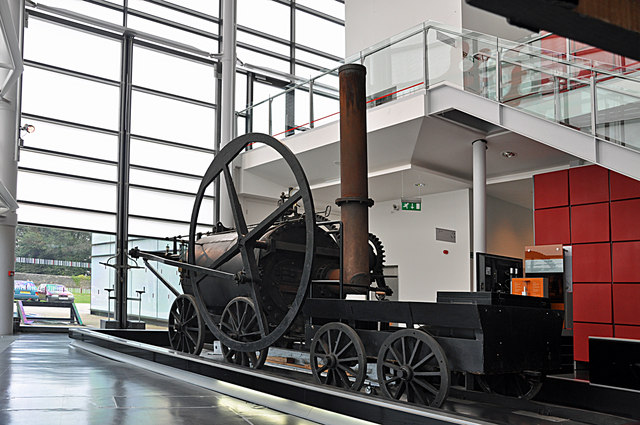
\includegraphics[width=.9\textwidth]{pen-y-darrenEngine.jpg}
\end{center}
\end{frame}

\begin{frame}
\frametitle{Blast furnaces 1709 (coke),\\ Blists Hill, Coalbrookdale, Shropshire}
\begin{center}
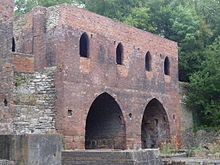
\includegraphics[height=.8\textheight]{blastFurnace.jpg}
\end{center}
\end{frame}

\begin{frame}
\frametitle{My interests}
\begin{itemize}
\item Long time background physics interest, bemusement over great divide \pause
\item Inet surfing (``unified field theory'' or ``TOE'') on $\bold{\uparrow}$ led me to Myron's site at least seven years ago \pause
\item The details on spacetime resonance energy (UFT87) completely hooked me as it fed my other passion \ldots \pause
\item Instead of retirement, I decided to complete my Ph.D. in economics to pursue $\left\lbrace \text{energy, development, growth}\right\rbrace$. \pause Along the way, I learned to ``surrender'' to the maths\pause
\item Last year I ``came out of the heterodox closet'' by writing Myron on cold fusion; I am humbled by the response and truly feel I am on the sidelines of a revolution\pause
\item So, onto the importance of energy in economic systems:
\footnote{A note on the University of Utah: one of the most heterodox economic programs in the world; also the home of Fleischmann and Pons experiments}
\end{itemize}
\end{frame}

\begin{frame}
\frametitle{English Industrial Revolution, 1590 - 1876}

	\begin{itemize}
	\item Modern economic growth
	\item Unconstrained quantity of fossil carbon energy -- an \textit{energy} revolution (in fact two!) led by a demand revolution
	\item Little statistical space for institutional or cultural events -- except to explain structural breaks
%	\item Framework applicable across time series, space, and time
	\end{itemize}
\end{frame}

\section{main}

\begin{center}
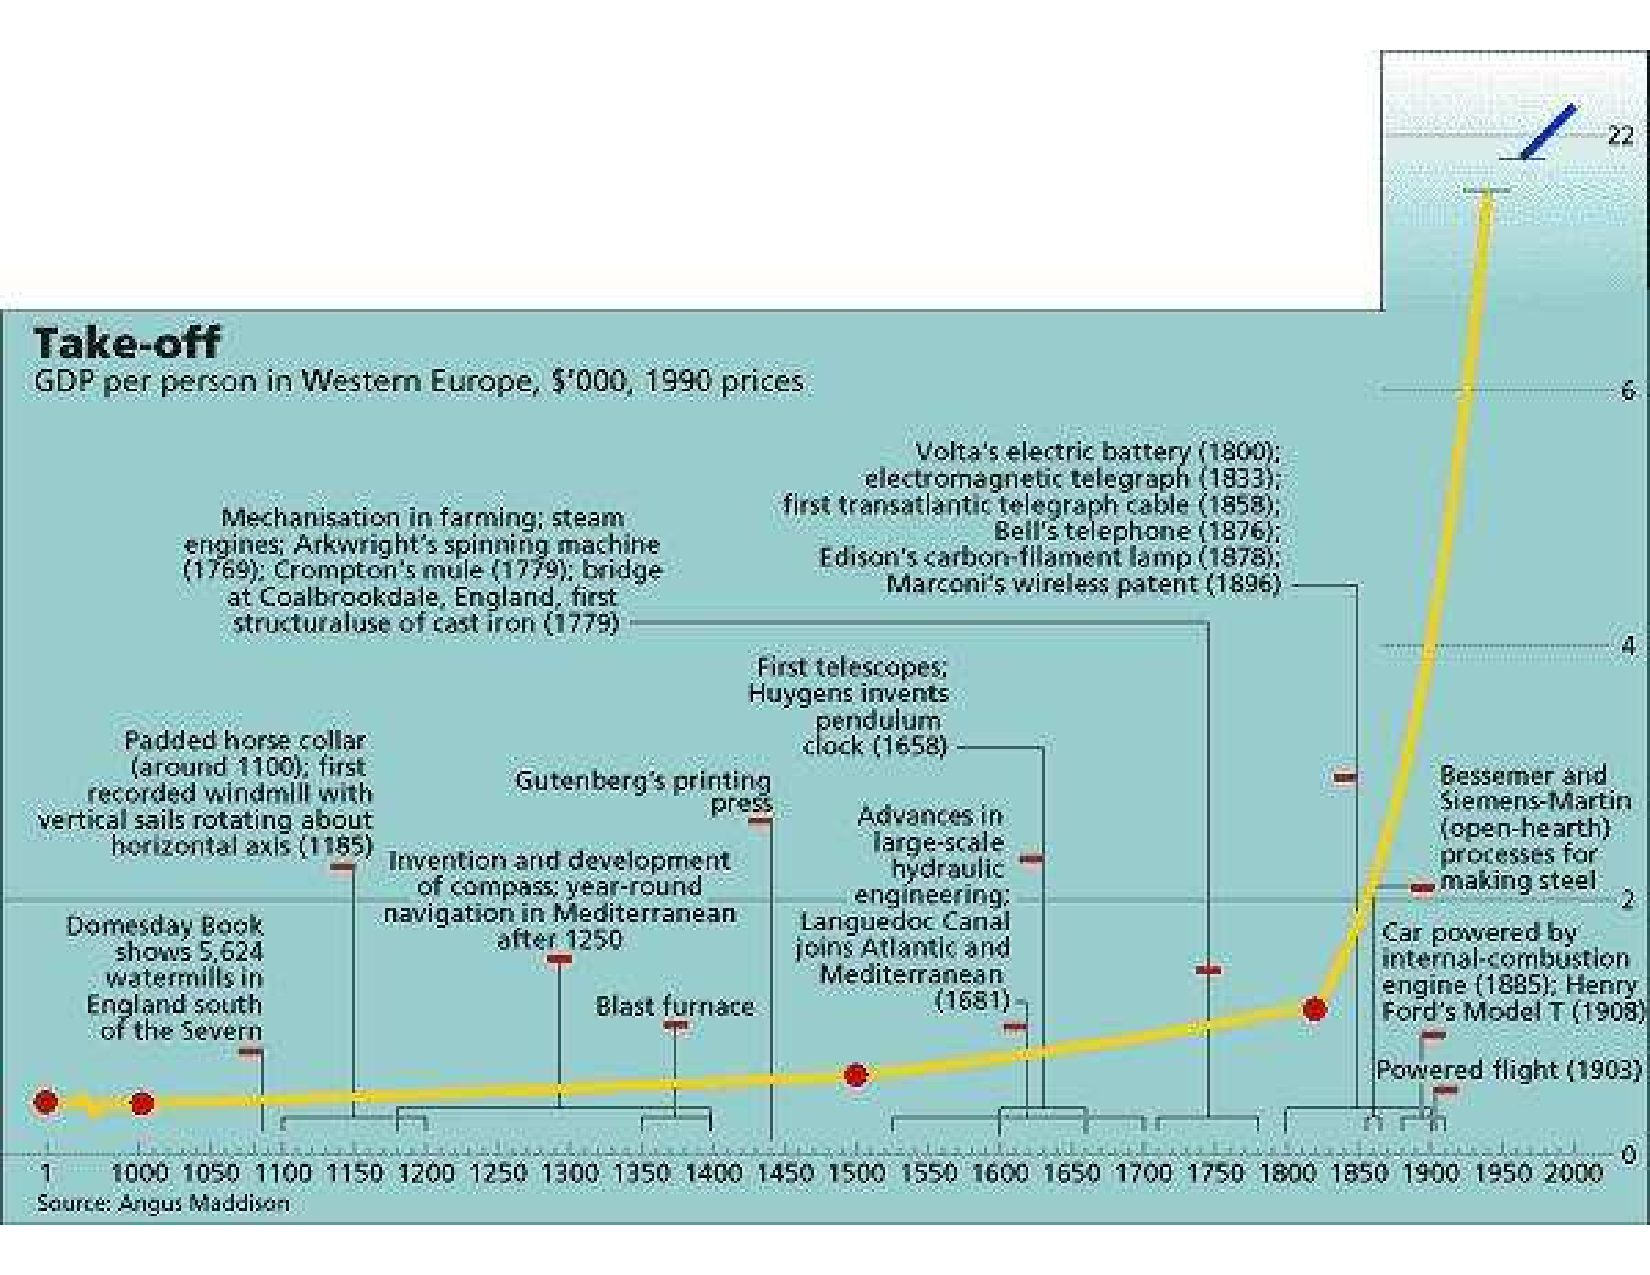
\includegraphics[width=0.99\textwidth]{roadtoriches.pdf}
\end{center}

\begin{frame}
\frametitle{Taxonomy of EIR explanations}
\footnotesize{
\begin{table}[p!]
%\caption{Taxonomy of EIR explanations}
\label{tbl:taxonomy}
\scriptsize{
\begin{tabular}{ll}
Label&Examples\\
\hline \hline
English exceptionalists&Landes (1969), McCloskey (2010), Mokyr (1992,2010)\\
Partial culturalists&Cipolla (1966), Pomeranz (2001), Allen (2009)\\
Primarily energetic&Cottrell (1955), Wrigley (1988,2010), Malanima (2010), Nef (1932)\\
Thermodynamicists&Georgescu-Roegen (1975), Ayres (2003), Garrett (2009)\\
\end{tabular}
}
\end{table}
}
\end{frame}

\begin{frame}
\frametitle{Author/time-span series of energy consumption, GDP, and population}
\begin{figure}[p!]
\center
%\caption{Author/time-span series of energy consumption, GDP, and population}
\label{fig:overall levels}
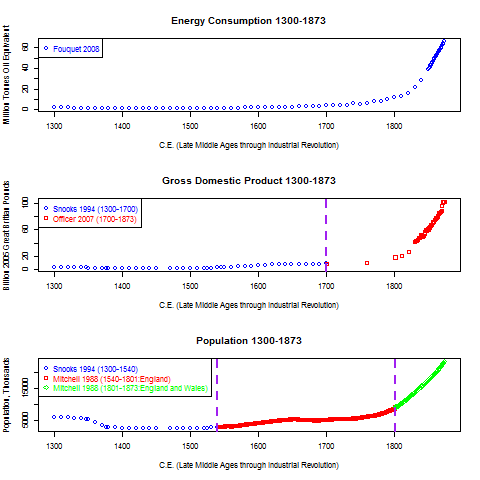
\includegraphics[height=0.8\textheight]{overallLevels}
\end{figure}
\end{frame}

\begin{frame}
\frametitle{English real gross domestic product, \\
levels and per--capita }

		\begin{figure}[p!]
%		\caption{English real gross domestic product, \\
%		levels and per--capita }
		\label{fig:ggdp}		
		\centerline{
		\mbox{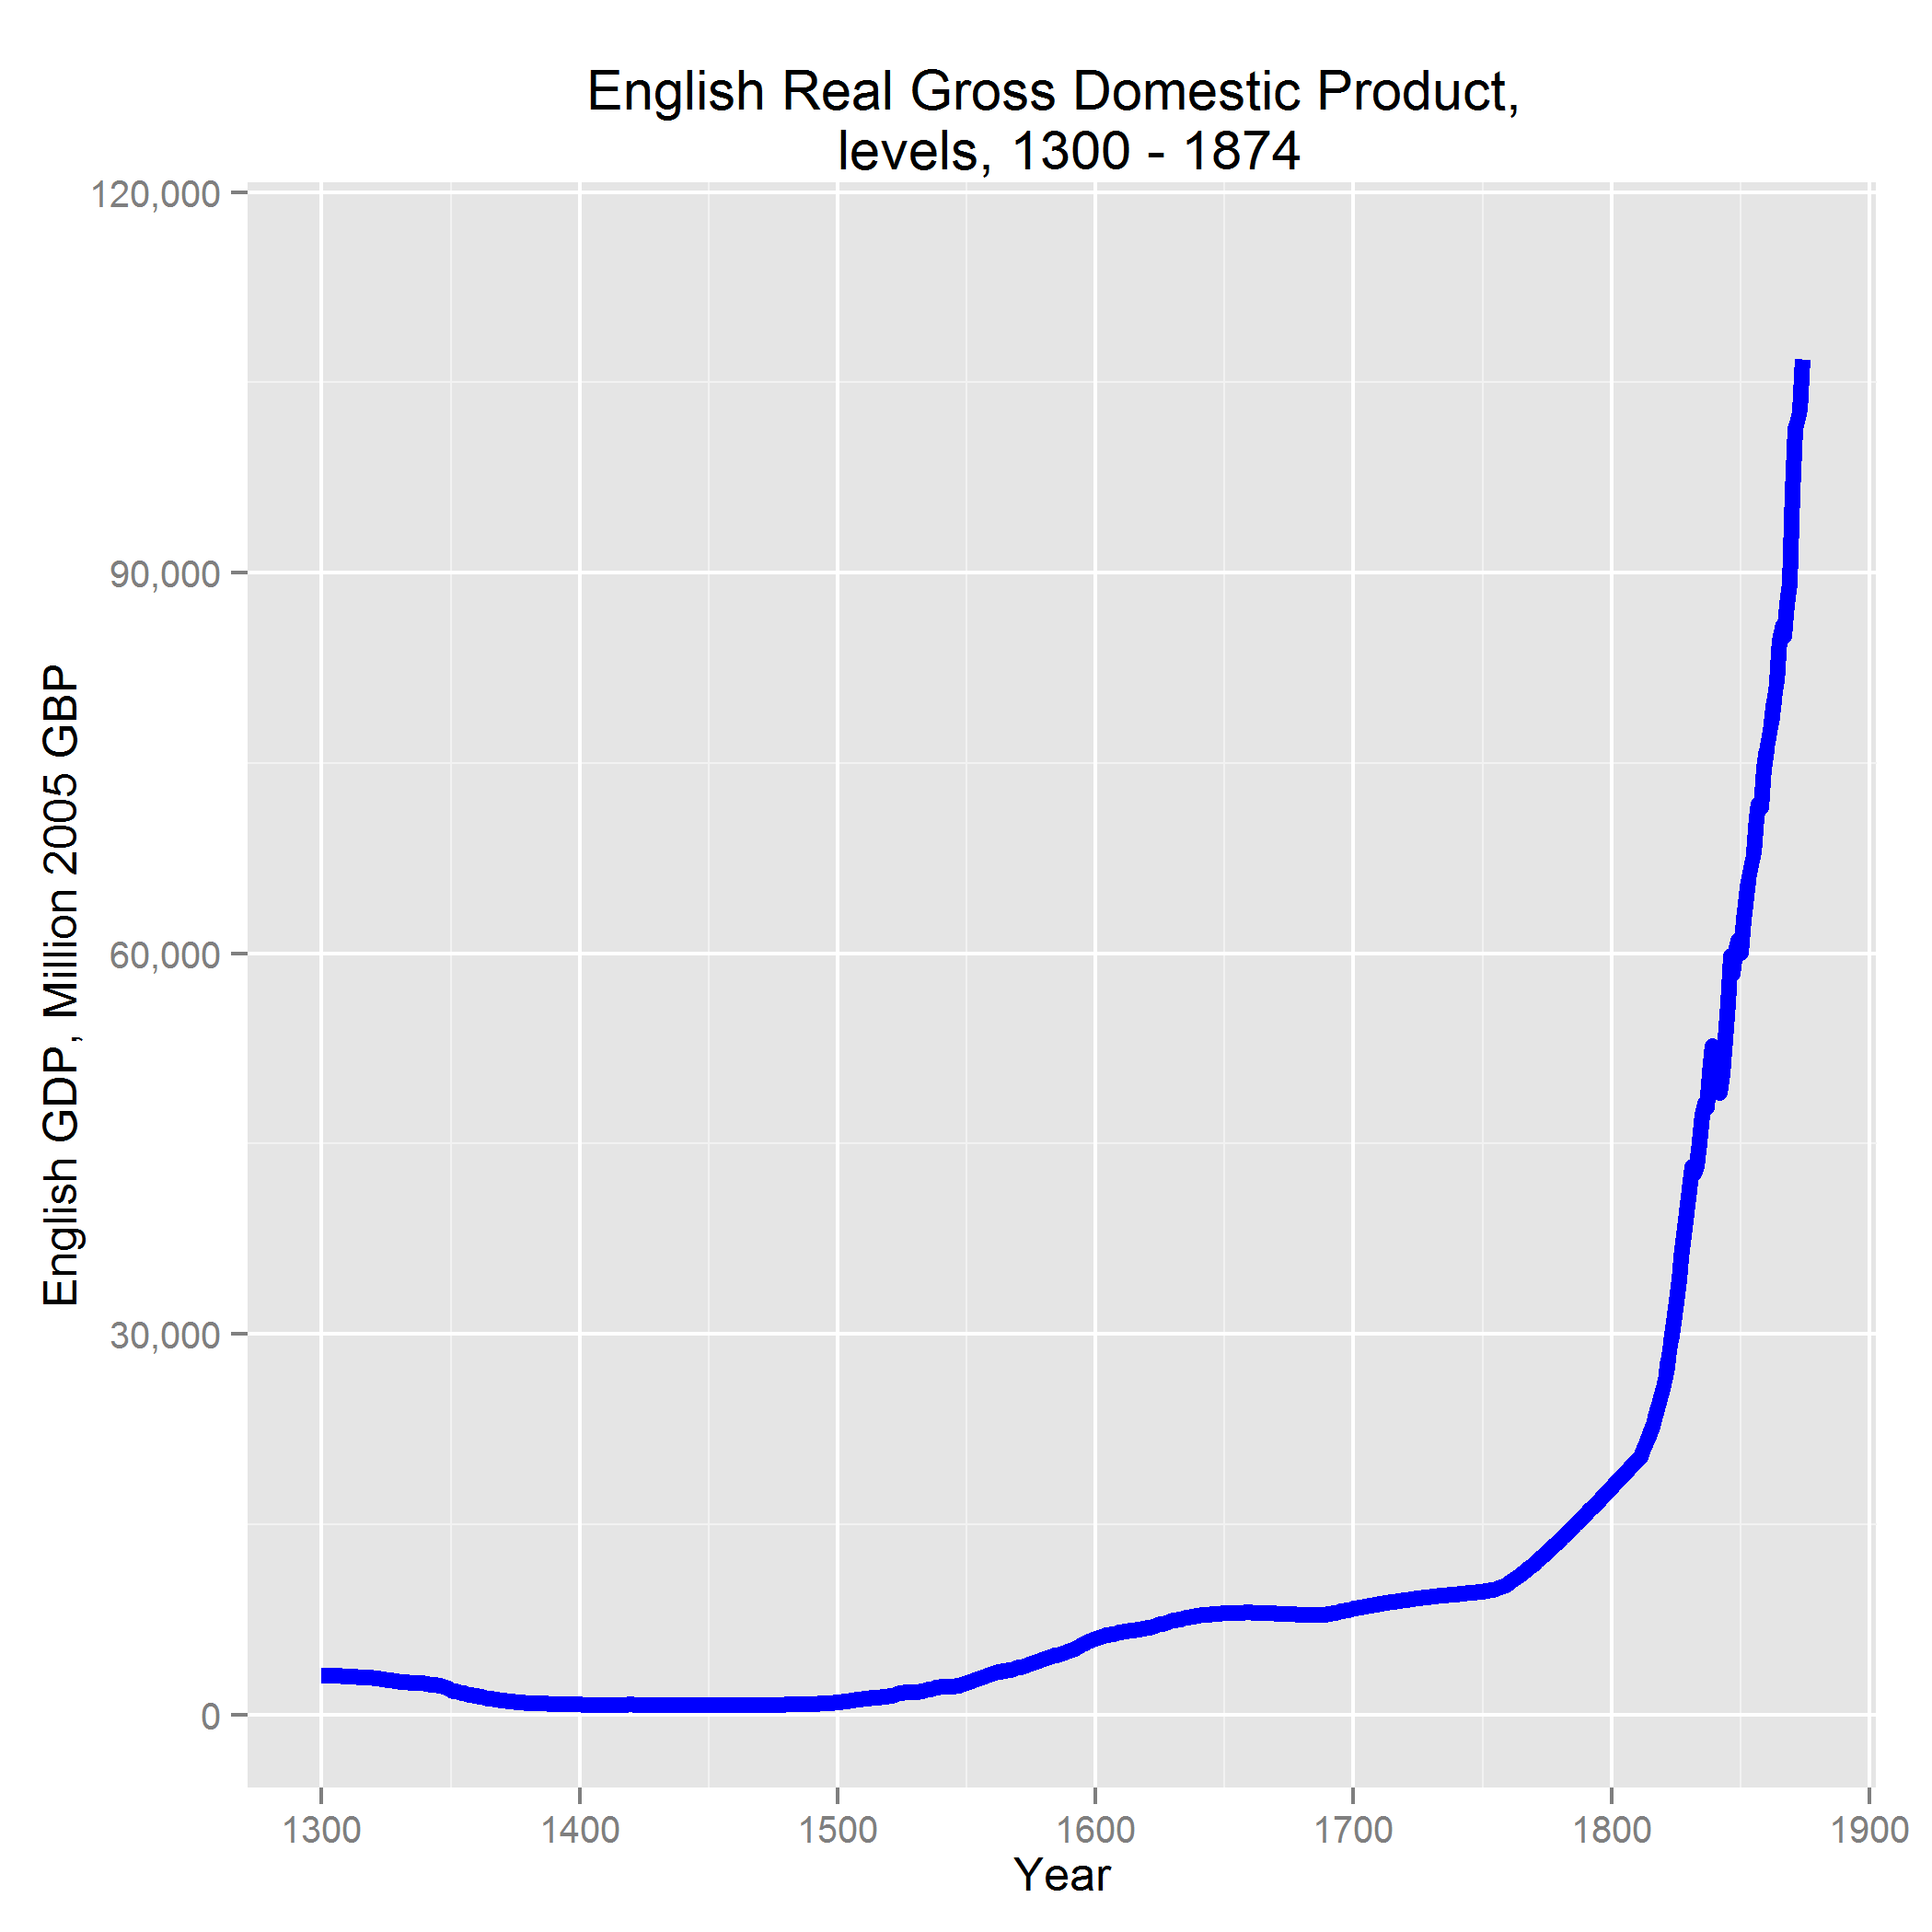
\includegraphics[width=0.55\textwidth]{ggdp}}
		\mbox{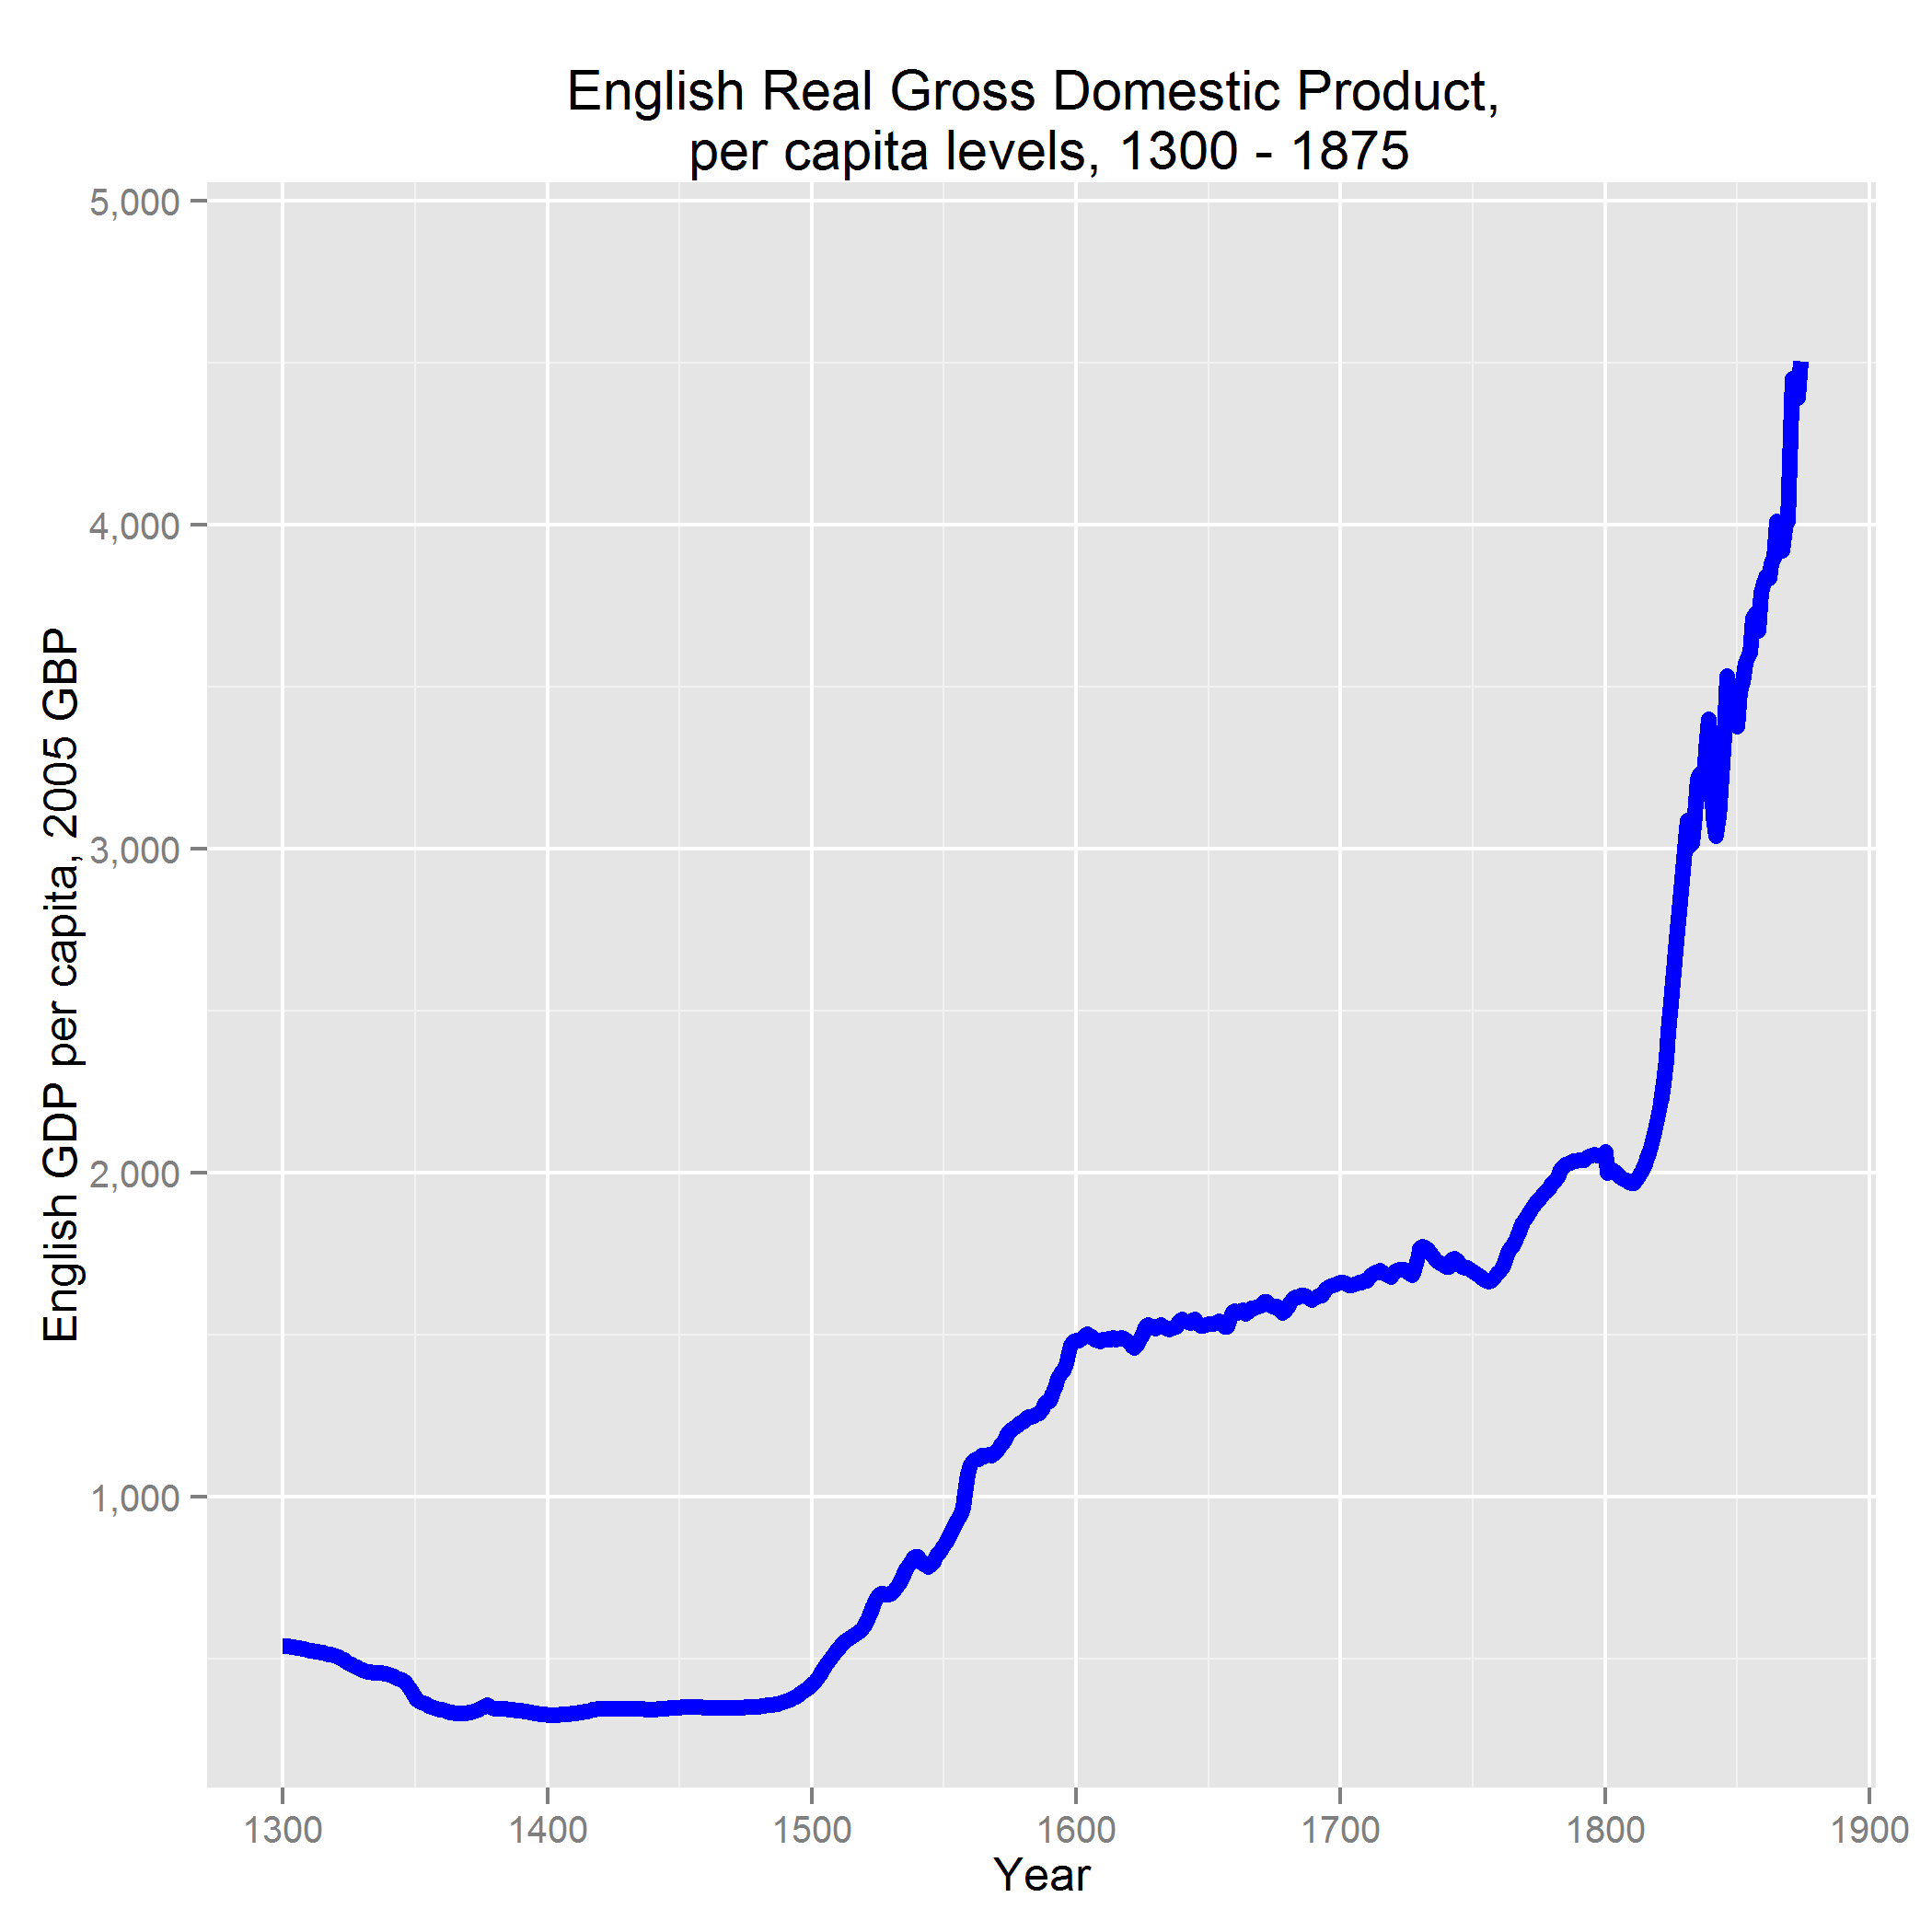
\includegraphics[width=0.55\textwidth]{ggdppop}}
		}
		\end{figure}
\end{frame}

\begin{frame}
		\frametitle{English real gross domestic product, \\
	log levels and log per--capita}

		\begin{figure}[p!]
%		\caption{English real gross domestic product, \\
%		log levels and log per--capita}
		\label{fig:gdpLog}		
		\centerline{
		\mbox{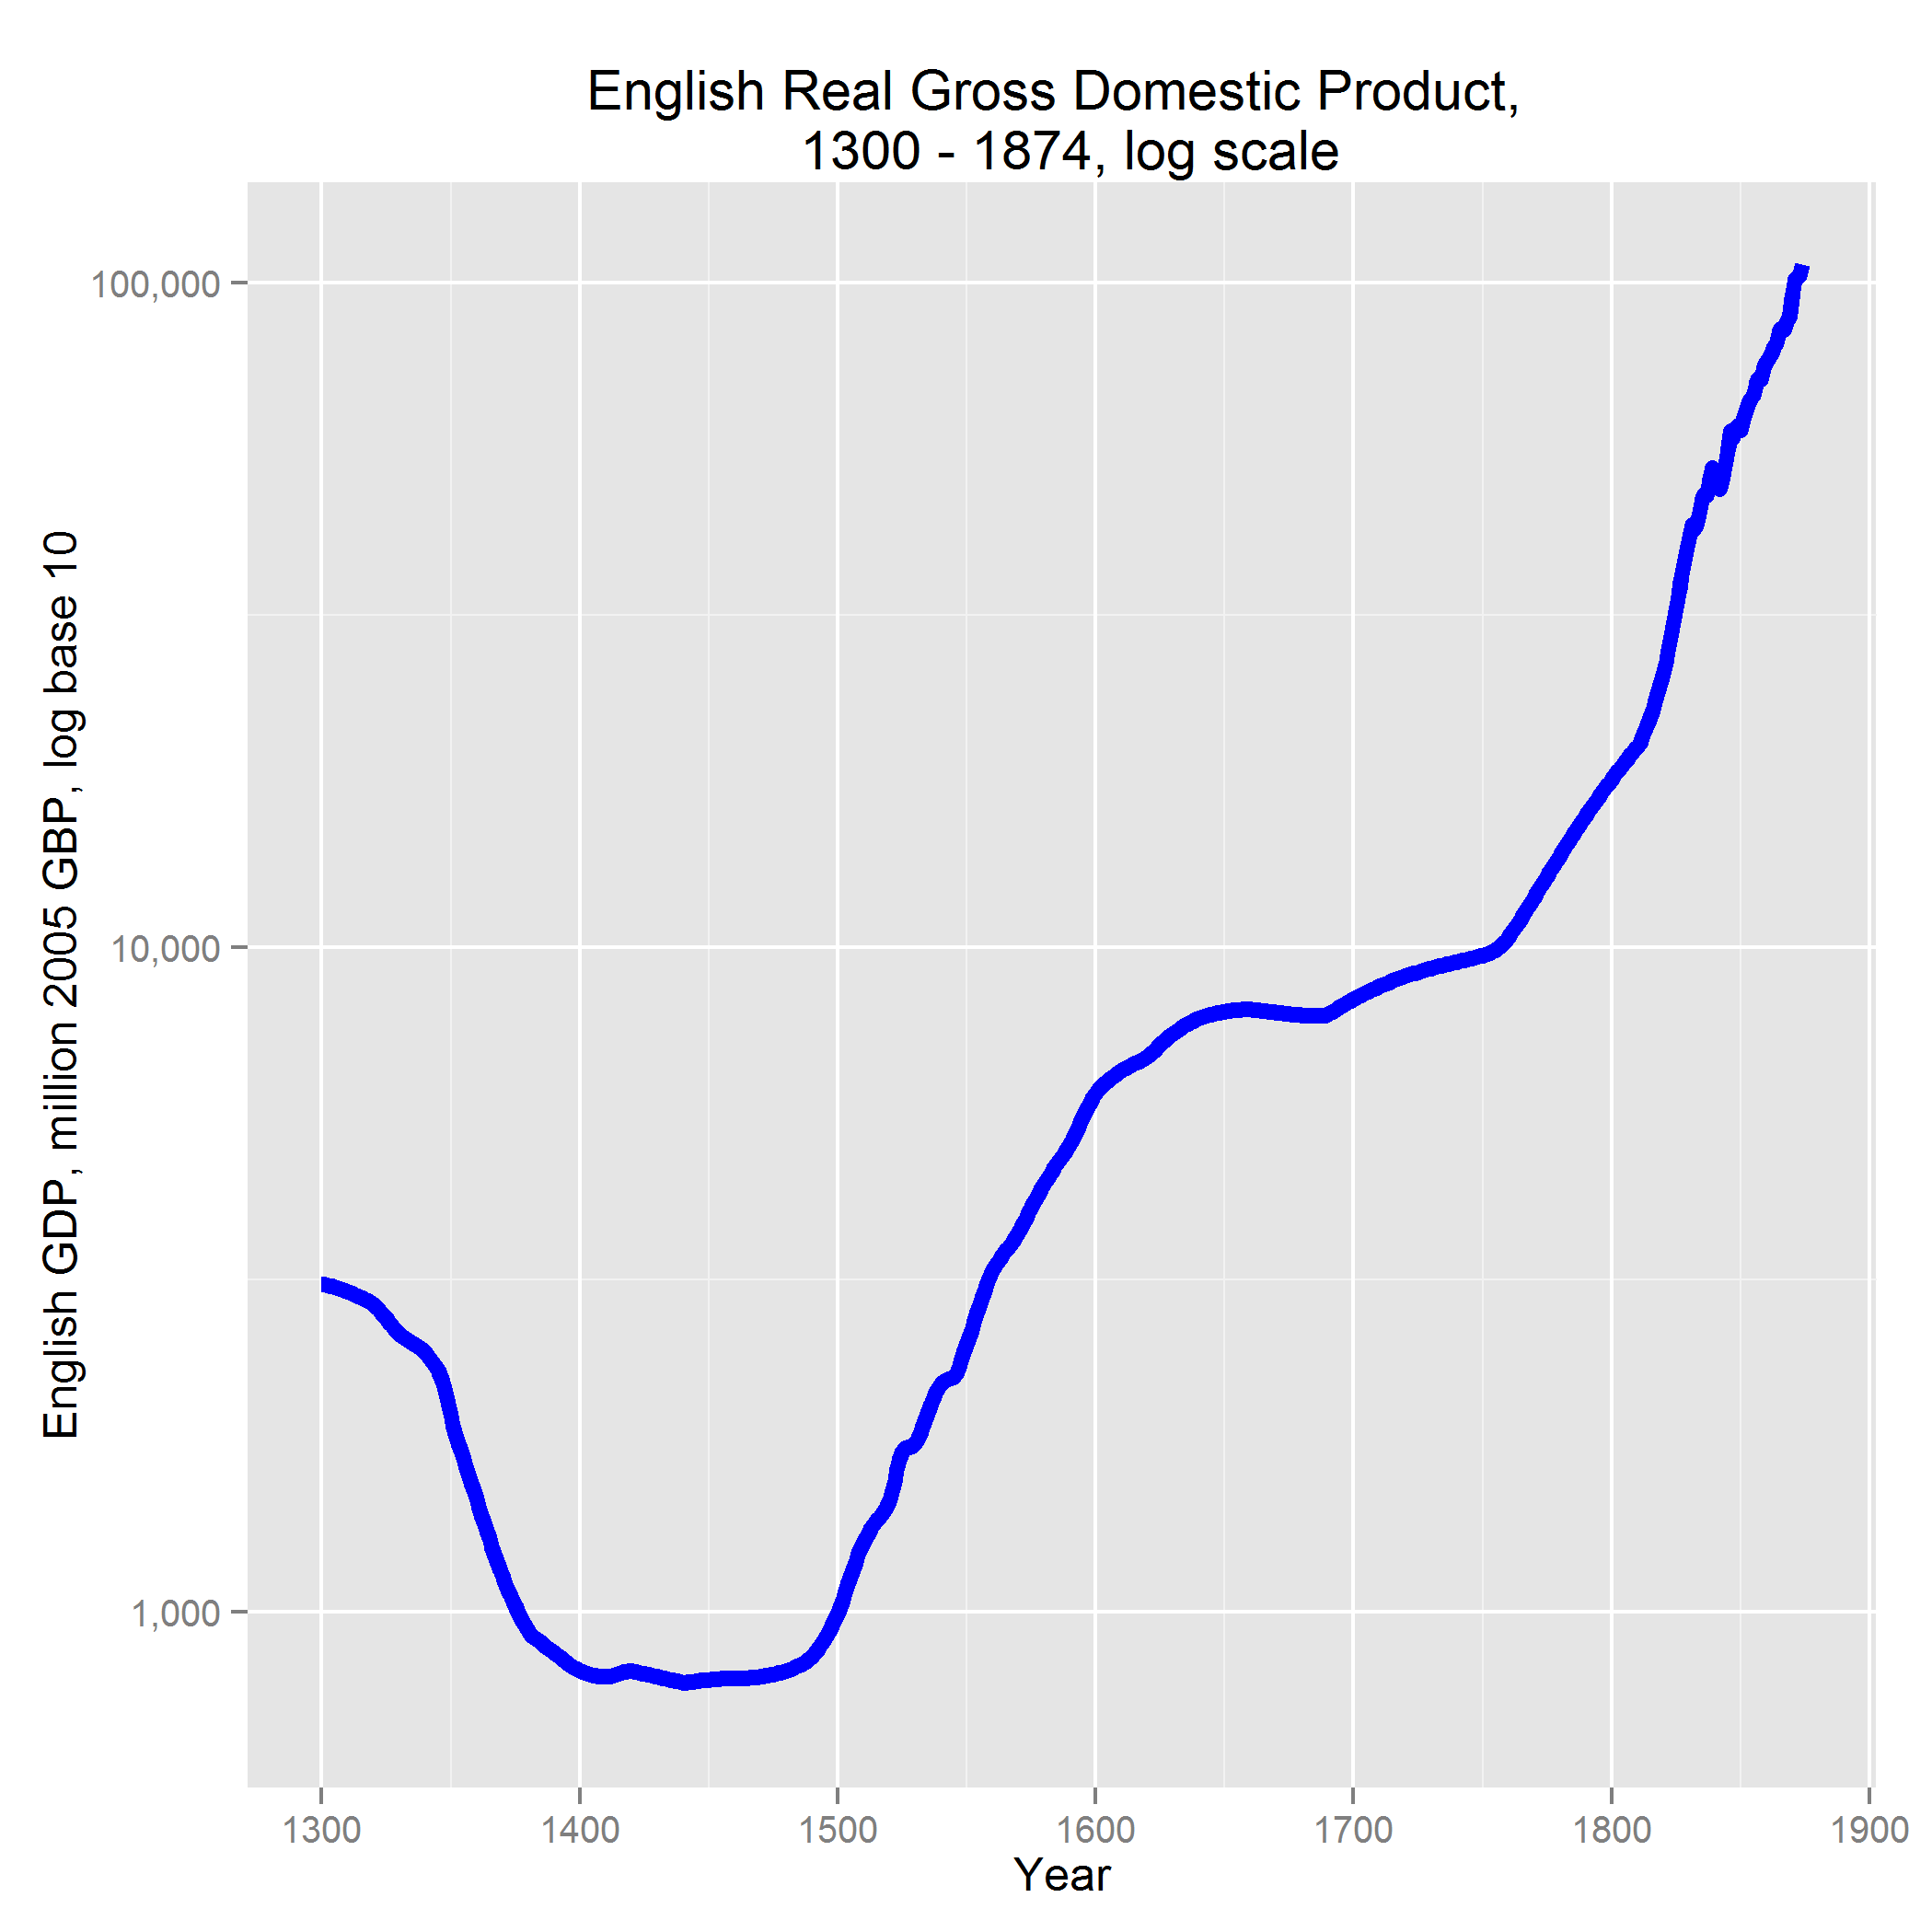
\includegraphics[width=0.55\textwidth]{gdpLog}}
		\mbox{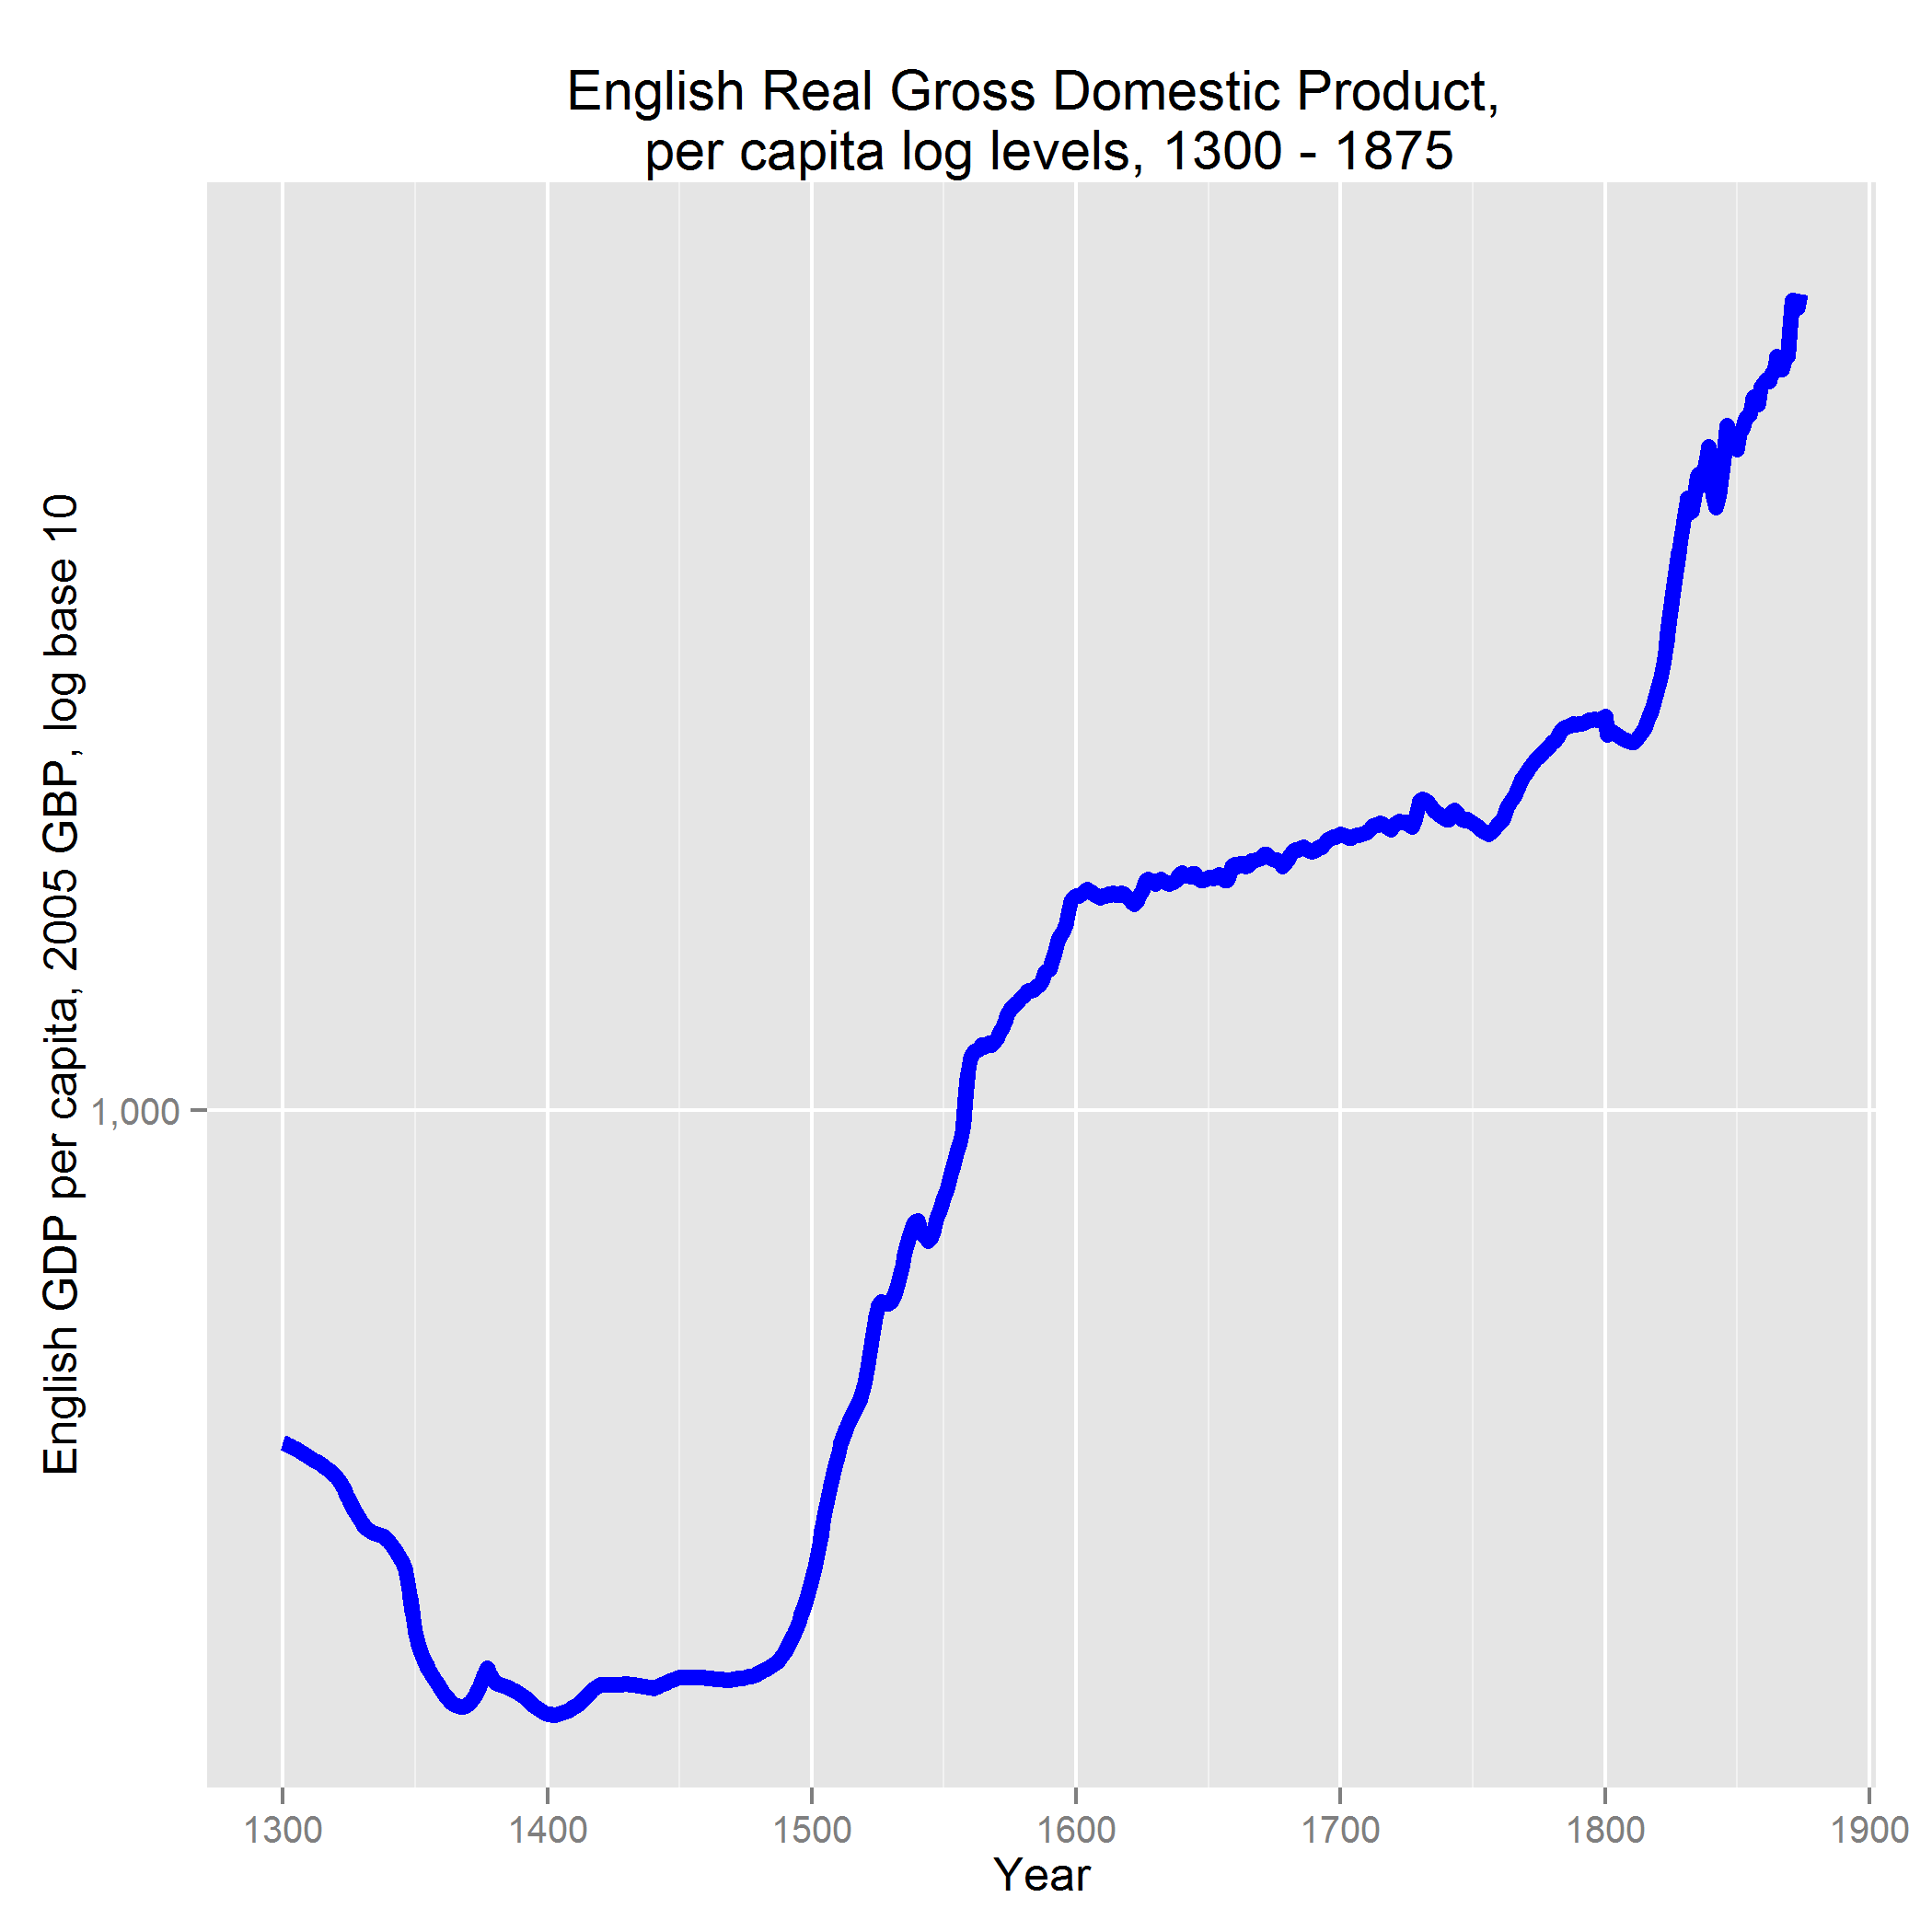
\includegraphics[width=0.55\textwidth]{gdpPopLog}}
		}
		\end{figure}
\end{frame}

\begin{frame}
		\frametitle{Structural break comparison}
\begin{figure}[p!]
%		\caption{Structural break comparison}
		\label{fig:structural}		
		\centerline{
		\mbox{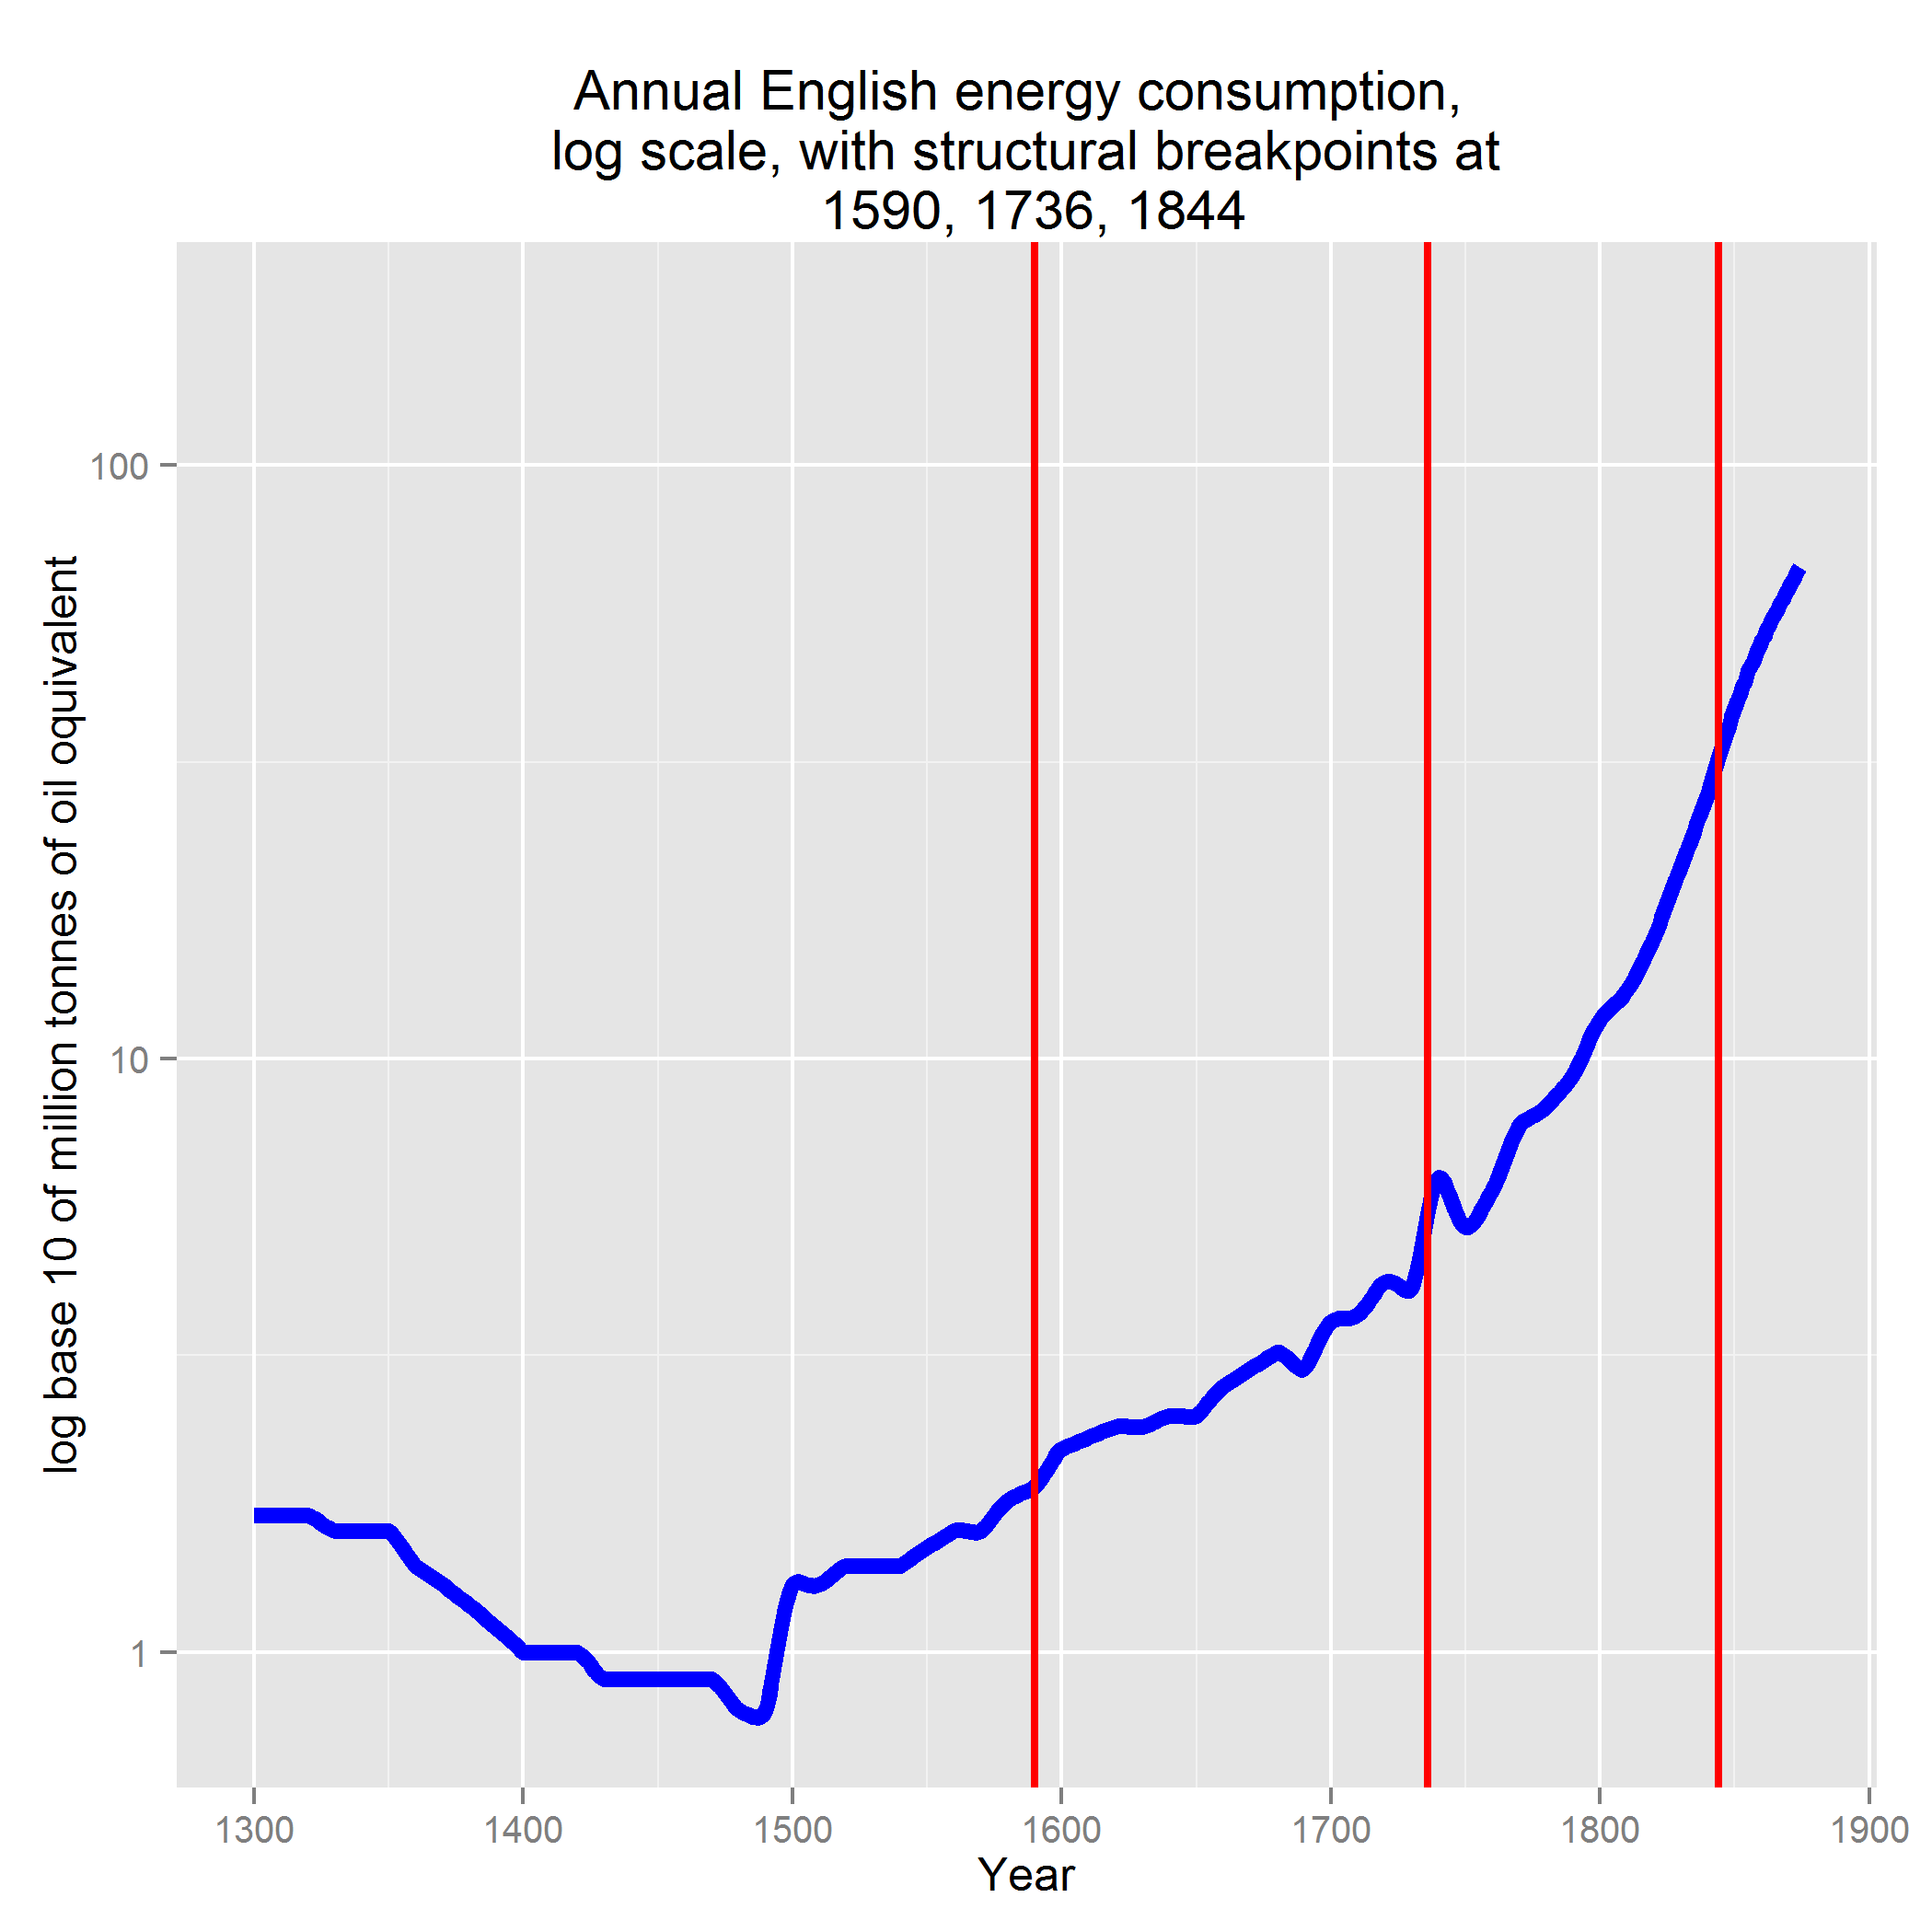
\includegraphics[width=0.39\textwidth]{energyLog1}}
		\mbox{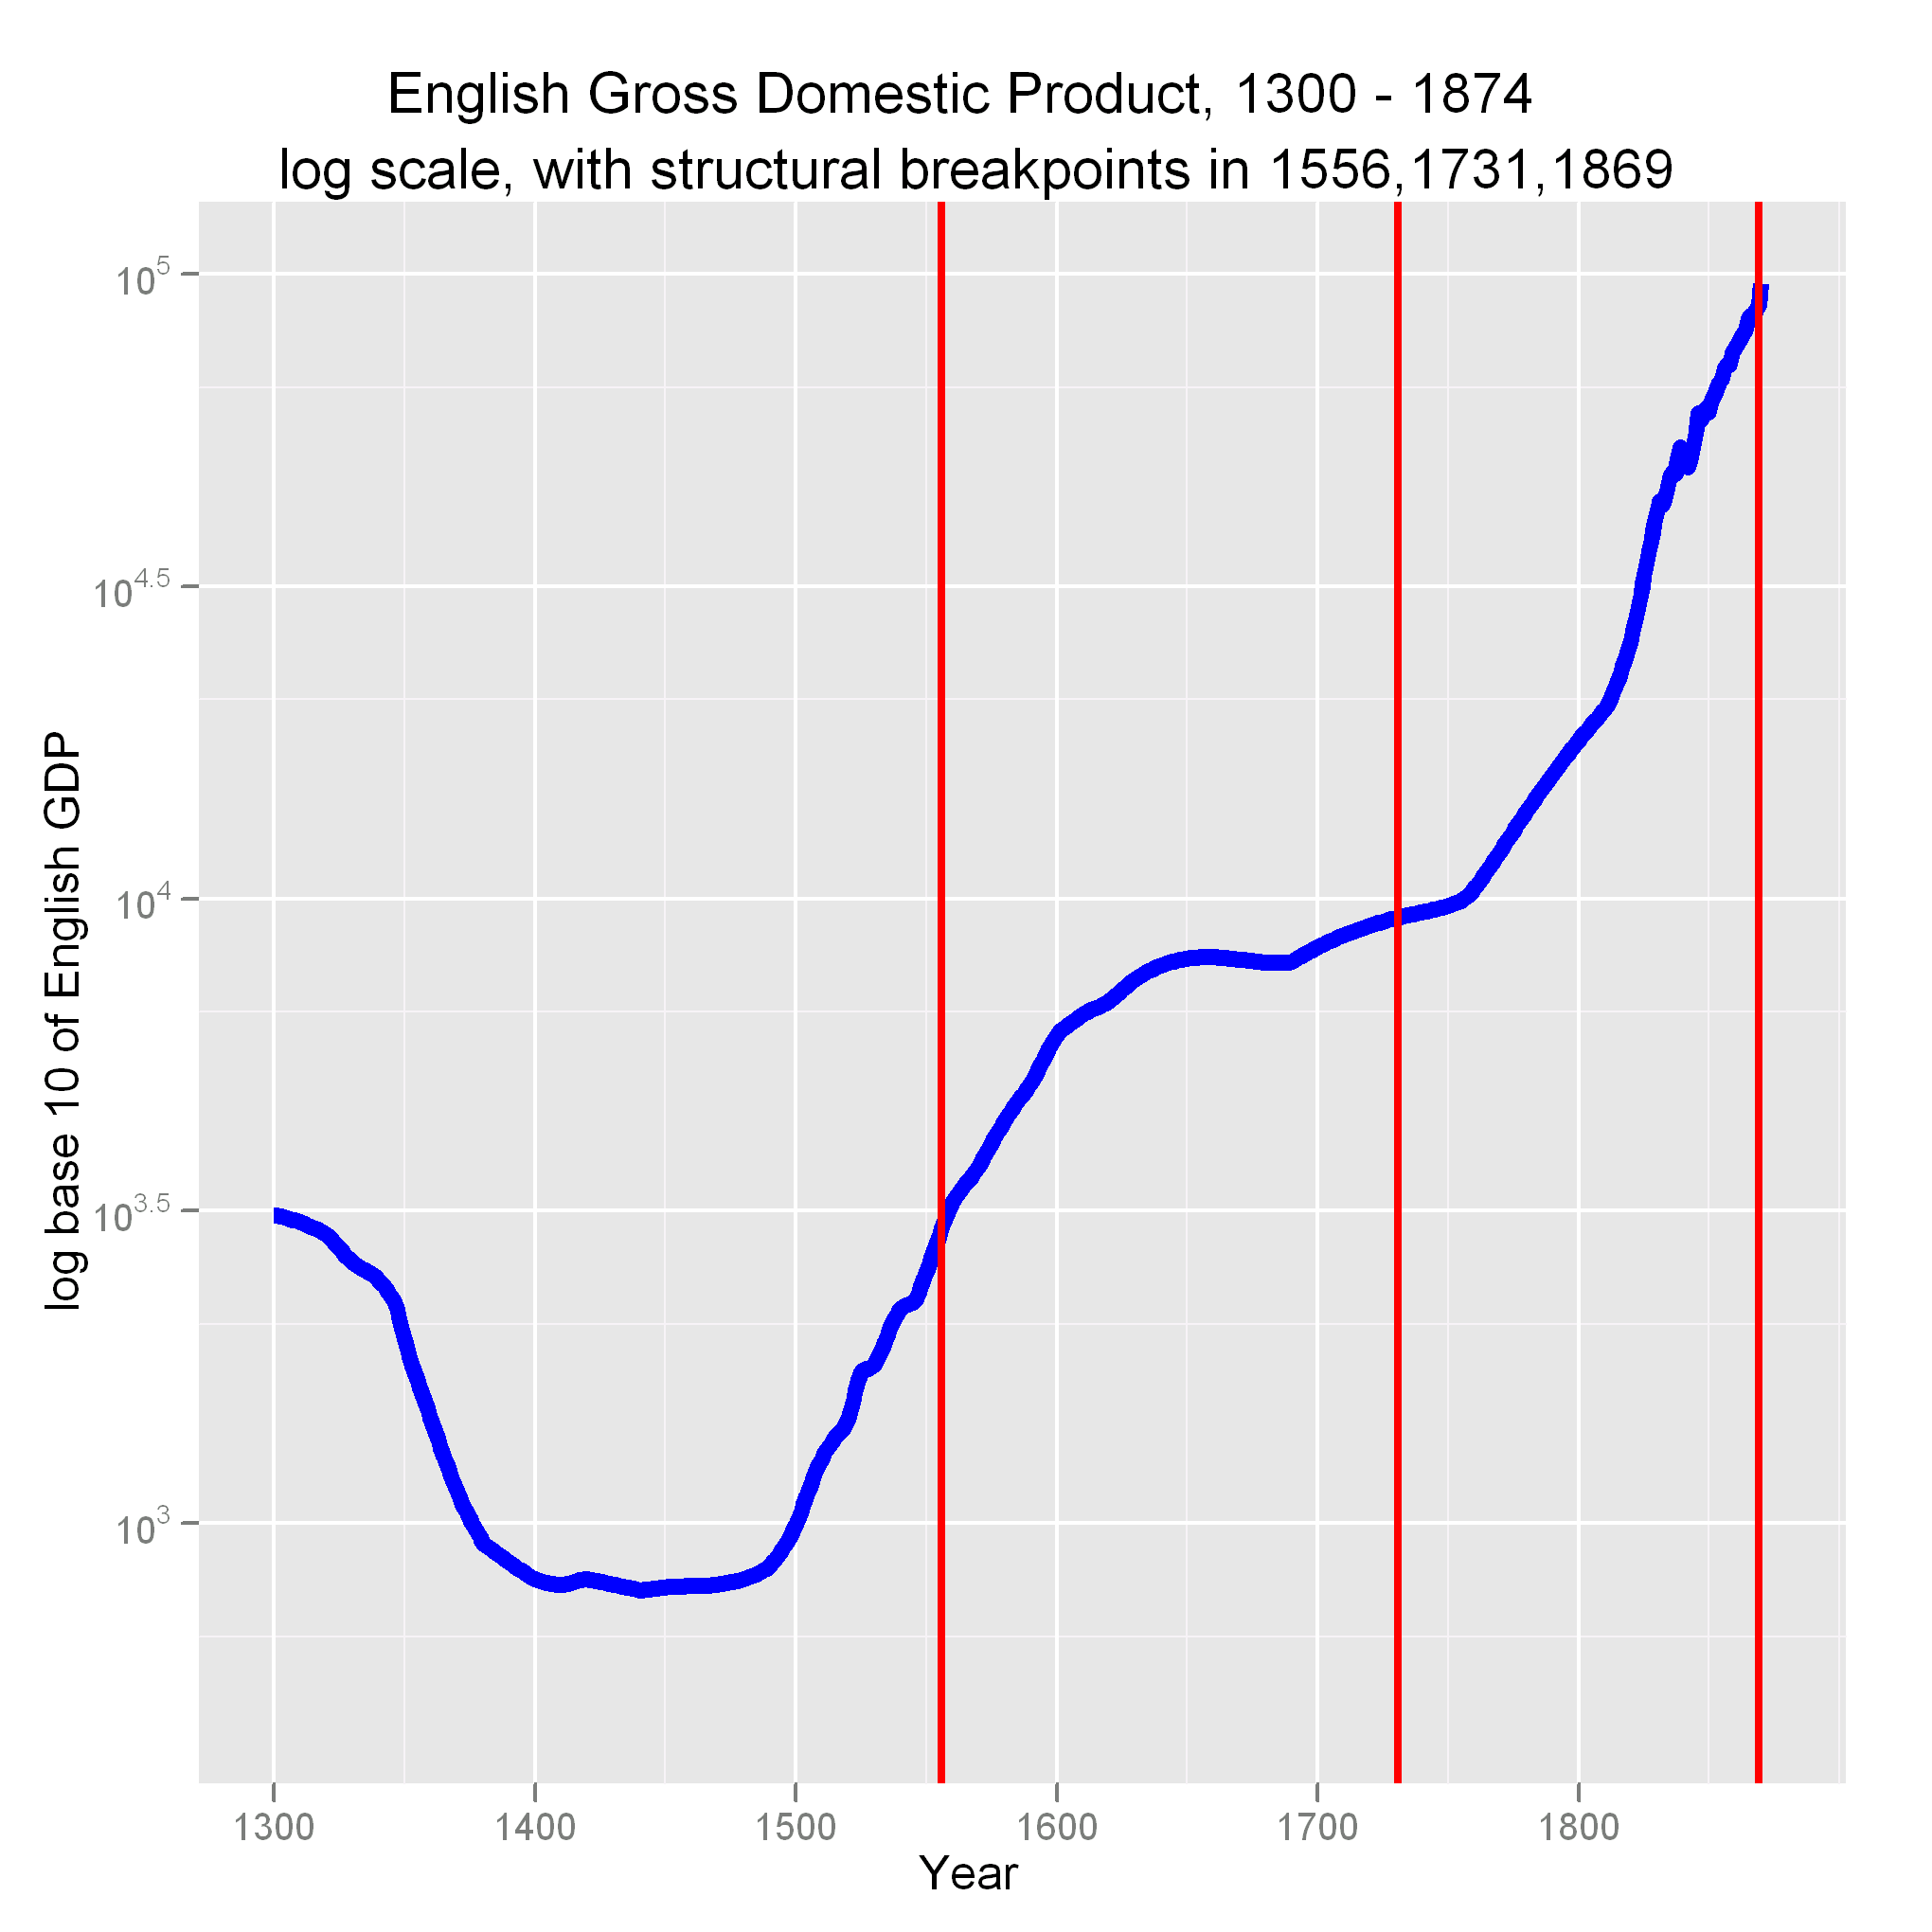
\includegraphics[width=0.39\textwidth]{gbpgdplog}}
		\mbox{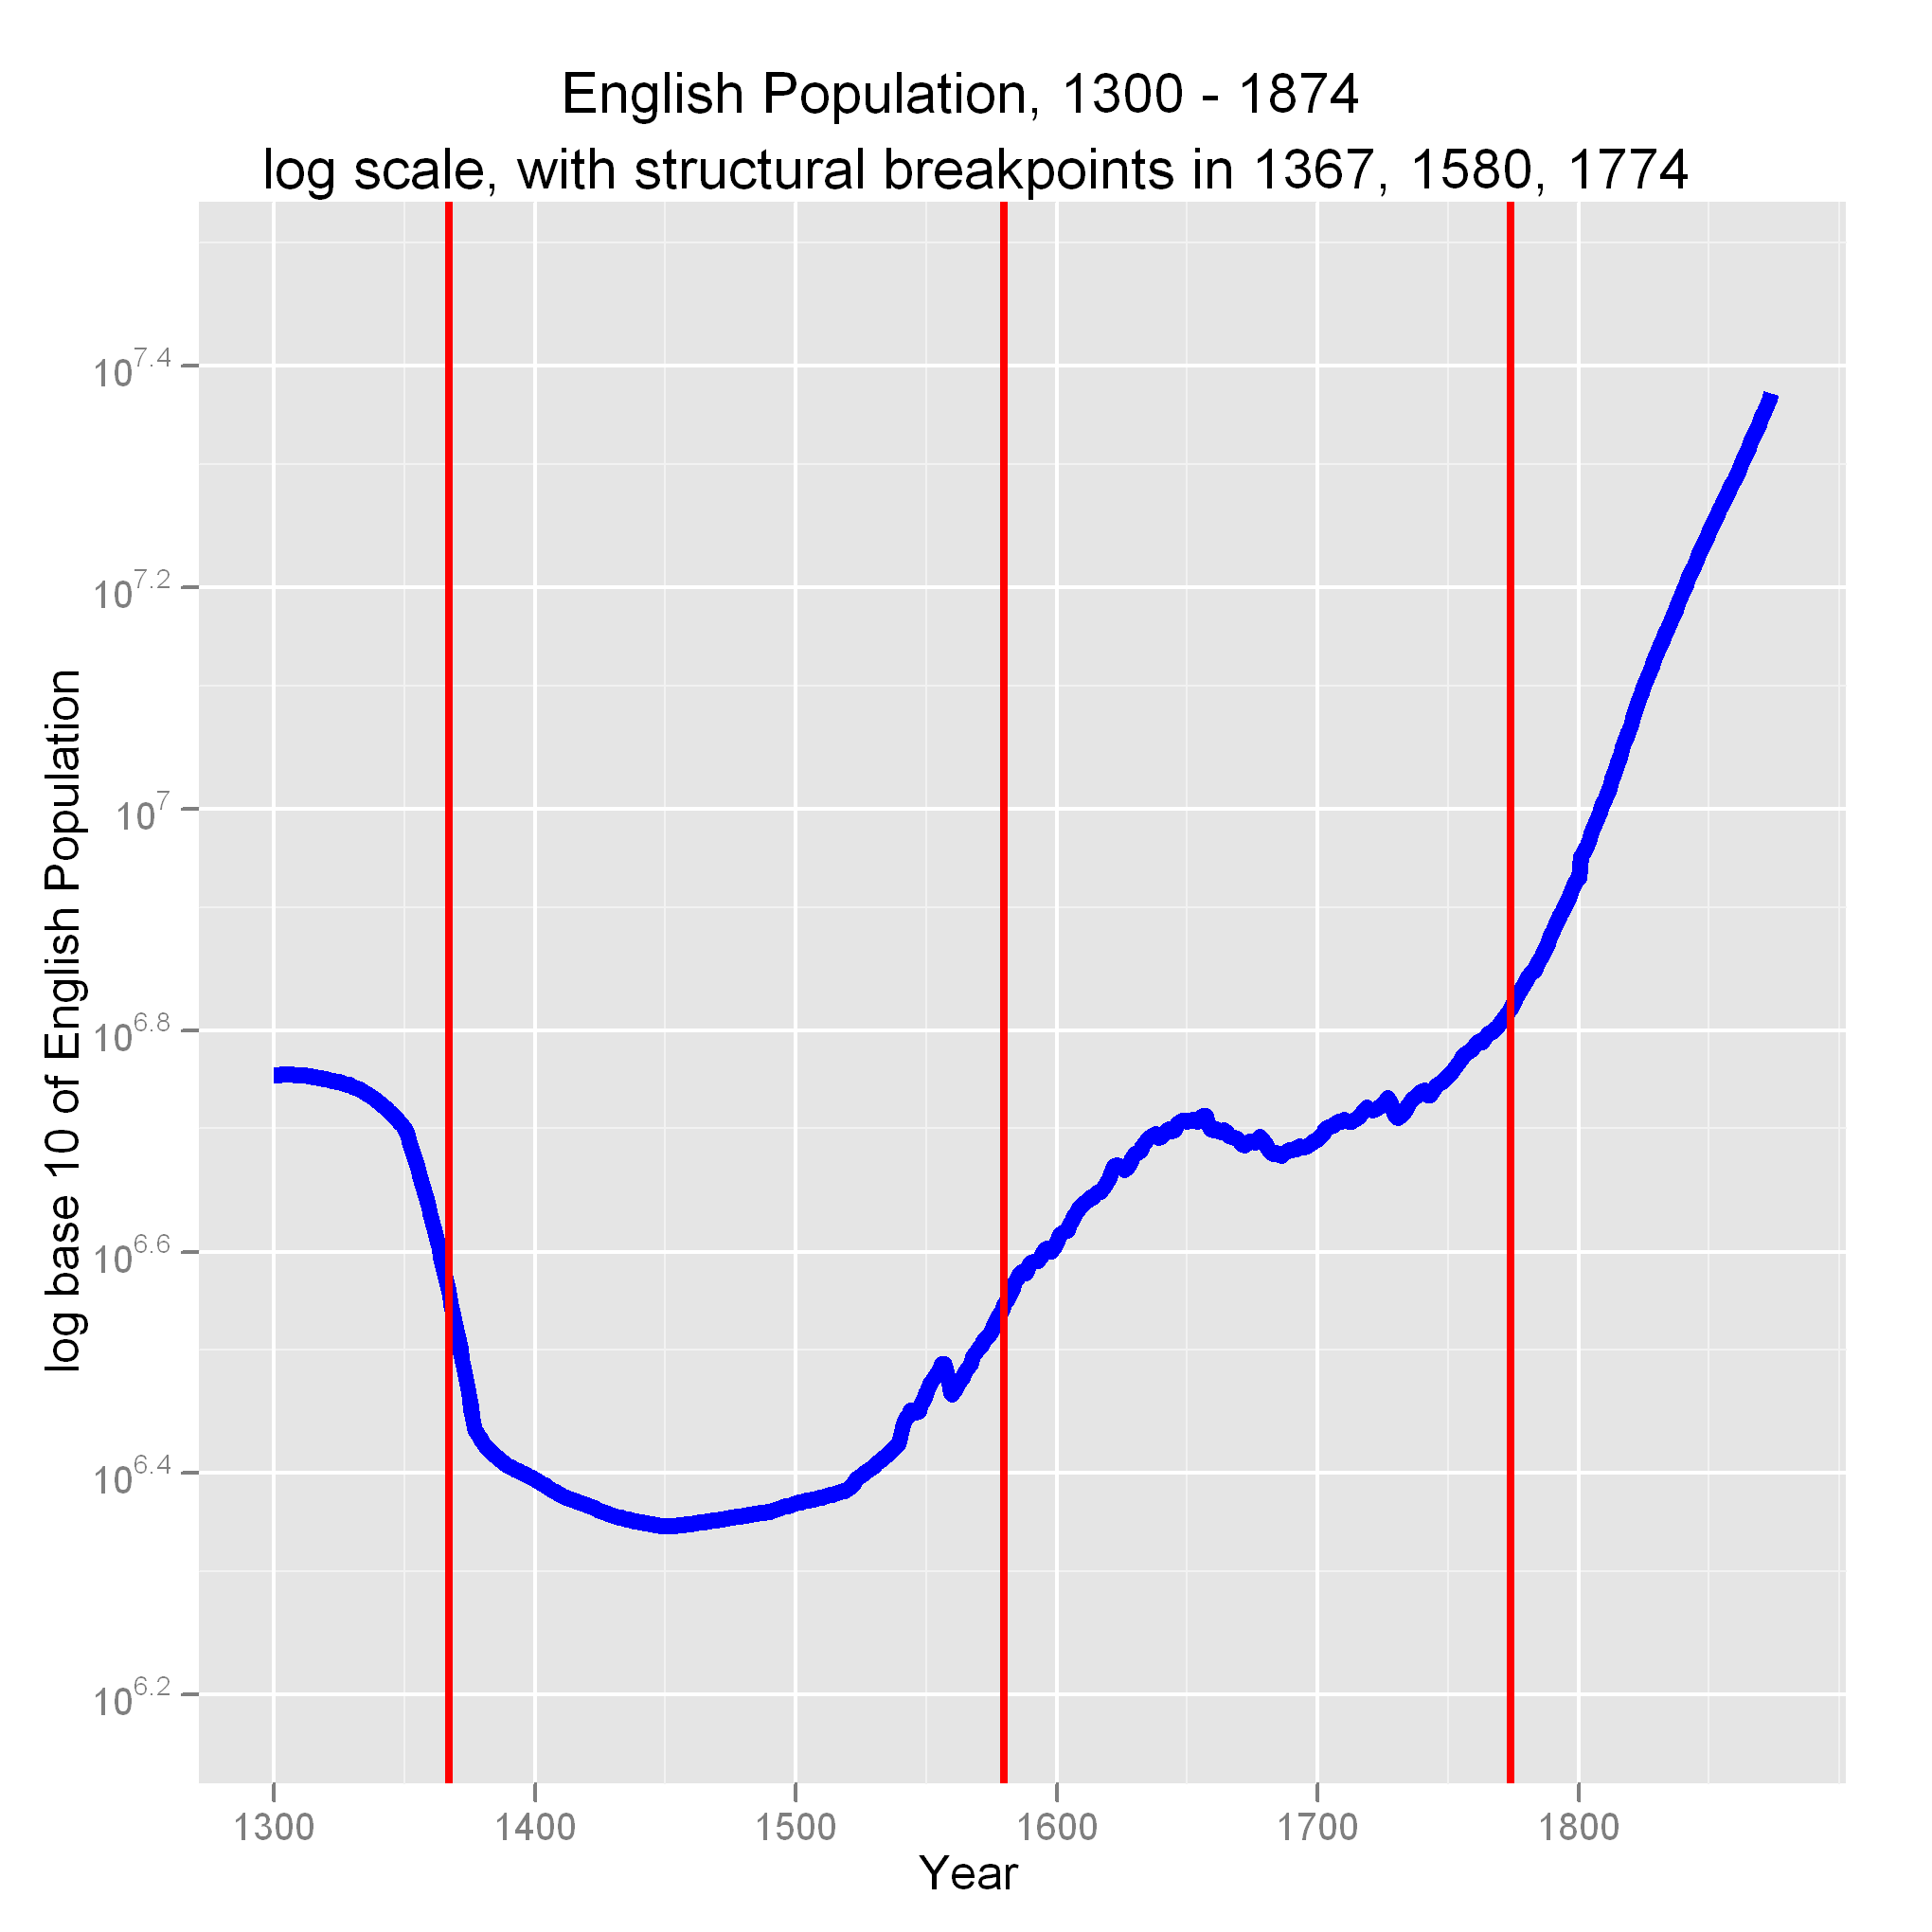
\includegraphics[width=0.39\textwidth]{popLog}}
		}
\end{figure}
\end{frame}

\begin{frame}
\frametitle{Coal and wood energy sources\\\textit{Source:} Pearson \& Fouquet}
\begin{figure}[p!]
\center
%\caption{Coal and wood energy sources\\\textit{Source:} Pearson \& Fouquet}
\label{fig:woodCoal}
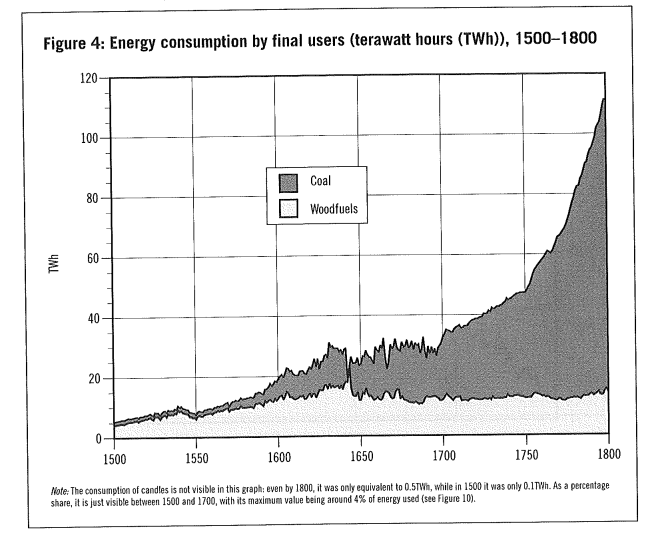
\includegraphics[height=0.8\textheight]{woodCoal.png}
\end{figure}
\end{frame}

\begin{frame}
\frametitle{Energy consumption vs. standarized GDP}
\begin{figure}[p!]
\center
%\caption{Energy consumption vs. standarized GDP}
\label{fig:energyVsGdp}
		\centerline{
		\mbox{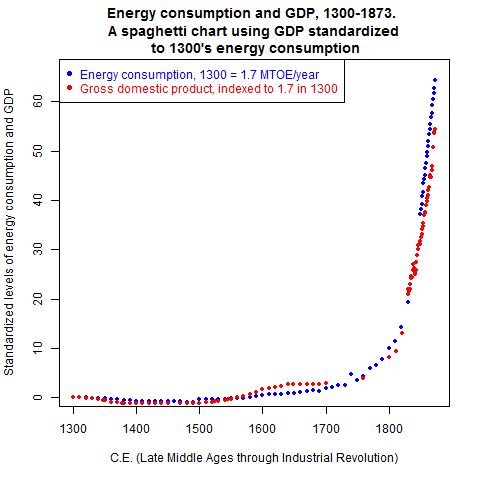
\includegraphics[width=0.55\textwidth]{energyVsGdp}}
		\mbox{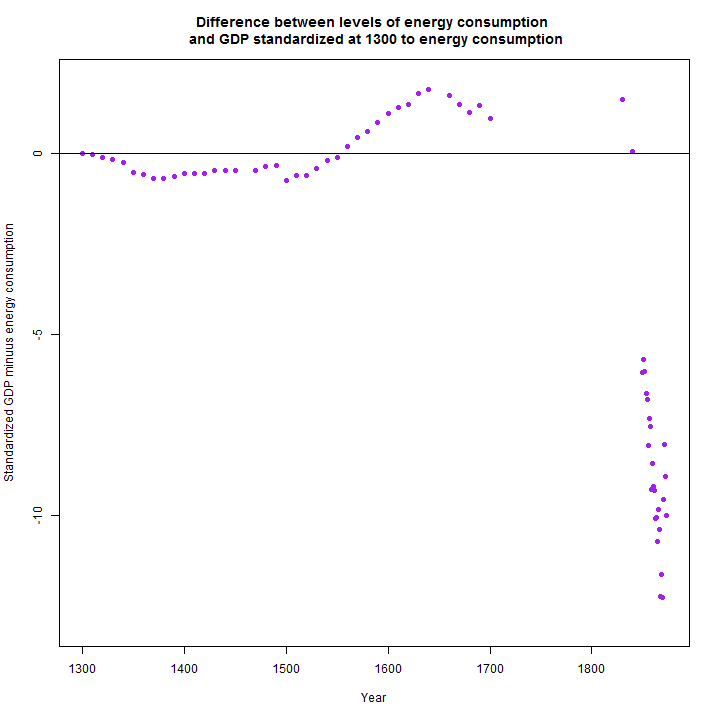
\includegraphics[width=0.55\textwidth]{energyVsGdpDiff}}
		}
\end{figure}
\end{frame}

\begin{frame}
\frametitle{Scatterplot of energy consumption vs. GDP}
\begin{figure}[p!]
\center
%\caption{Scatterplot of energy consumption vs. GDP}
\label{fig:scatterplot}
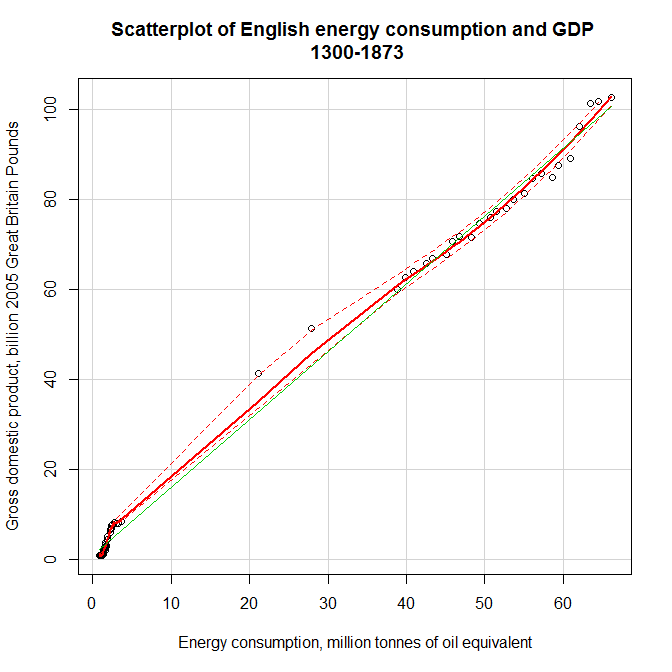
\includegraphics[height=0.8\textheight]{scatterplot.png}
\end{figure}
No ``Solow'' residual
\end{frame}

\begin{frame}
\frametitle{Granger tests of energy/GDP dynamics}
\scriptsize{
\begin{table}[p!]
%\caption{Granger tests of energy/GDP dynamics}
\label{tbl:grangerEnergyGdp}
\begin{tabular}{lrrl}
Era&Energy $\sim$ GDP Pr($>$F)& GDP $\sim$ Energy Pr($>$F)&AS/AD regime\\
\hline \hline
1300 -- 1500&0.0106&0.0003&EMP \footnote{European marriage pattern (Hajnal)}, Black Death: \\&&&increasing wages, \\
&&&family income\\
1500 -- 1600&0.1939&0.6126&Positive demand shock\\
1600 -- 1750&0.3529&0.5185&Energy supply constraint\\
1750 -- 1873&0.0024&0.1100&Positive supply shock:\\&&&``virtuous'' macro \\
&&&feedback cycle\\
\hline
1300 -- 1873& 0.0002& 0.0361&Total study period\\
\end{tabular}
\end{table}
}
\end{frame}

\begin{frame}
		\frametitle{Aggregate Supply - Aggregate Demand \\ Four energy/GDP regimes}
\begin{figure}[p!]
%		\caption{Aggregate Supply - Aggregate Demand \\ Four energy/GDP regimes}
		\label{fig:asad}		
		\centerline{
		\mbox{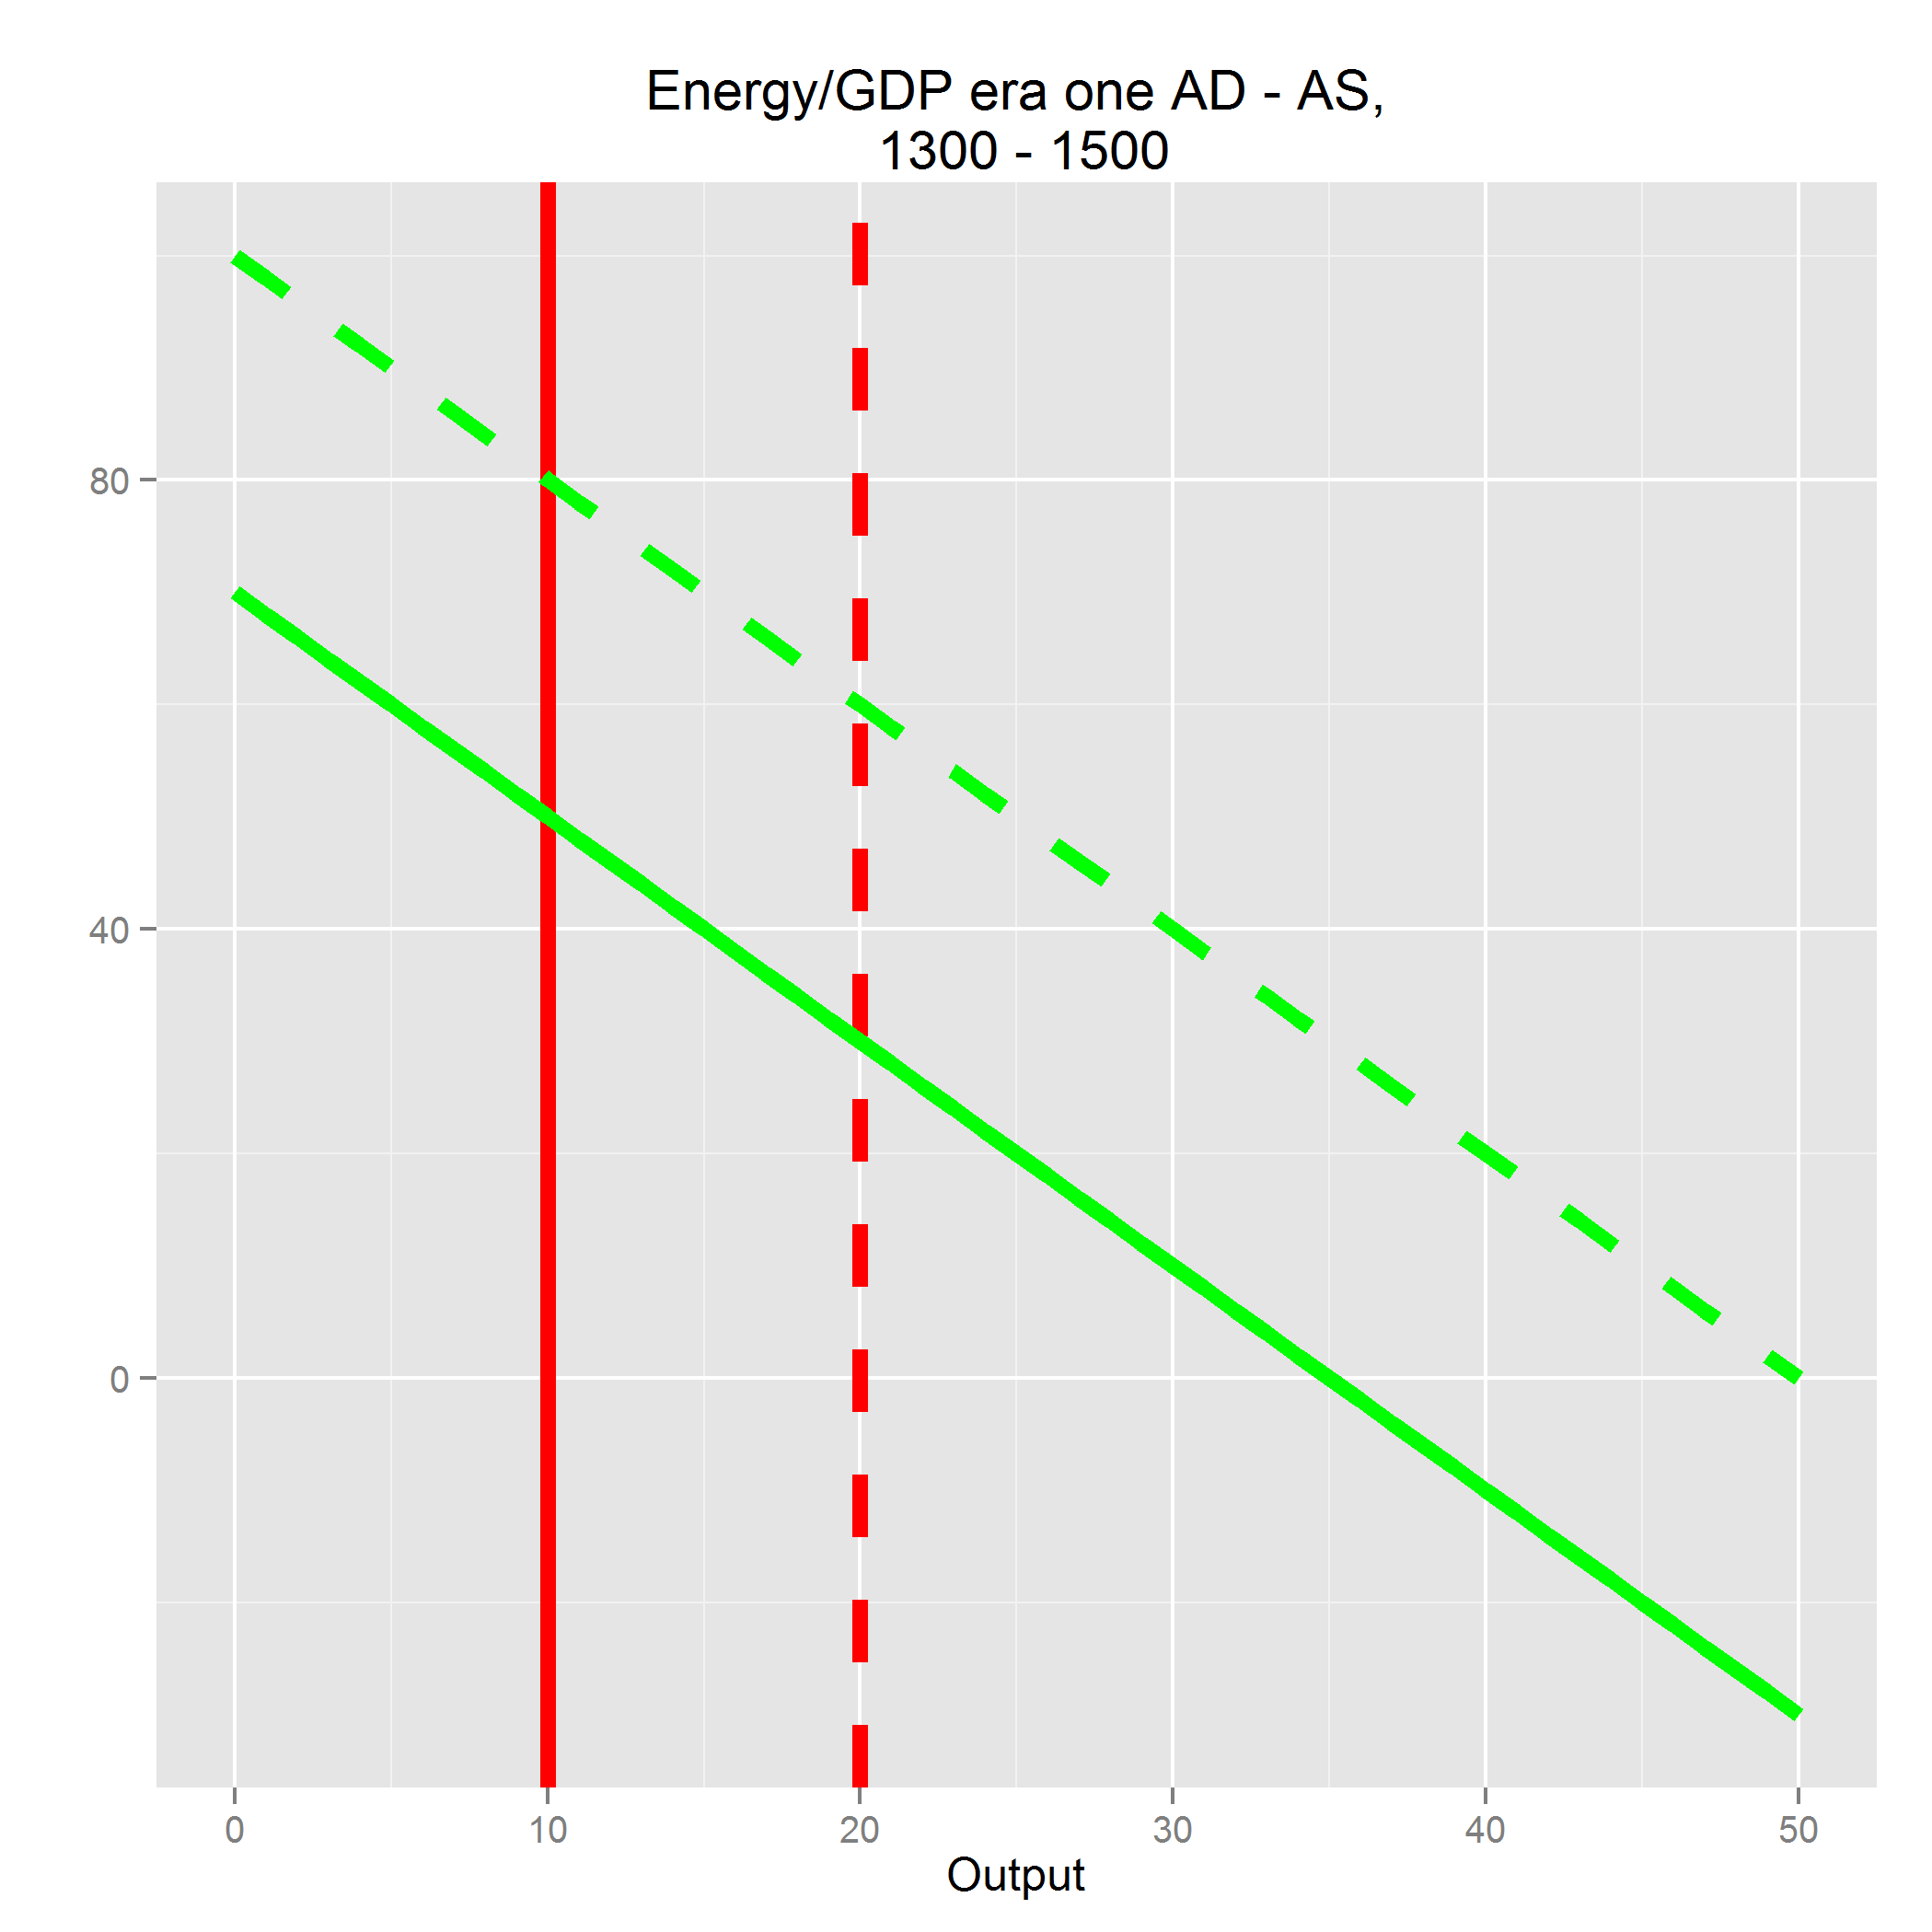
\includegraphics[height=0.35\textheight]{era1}}
		\mbox{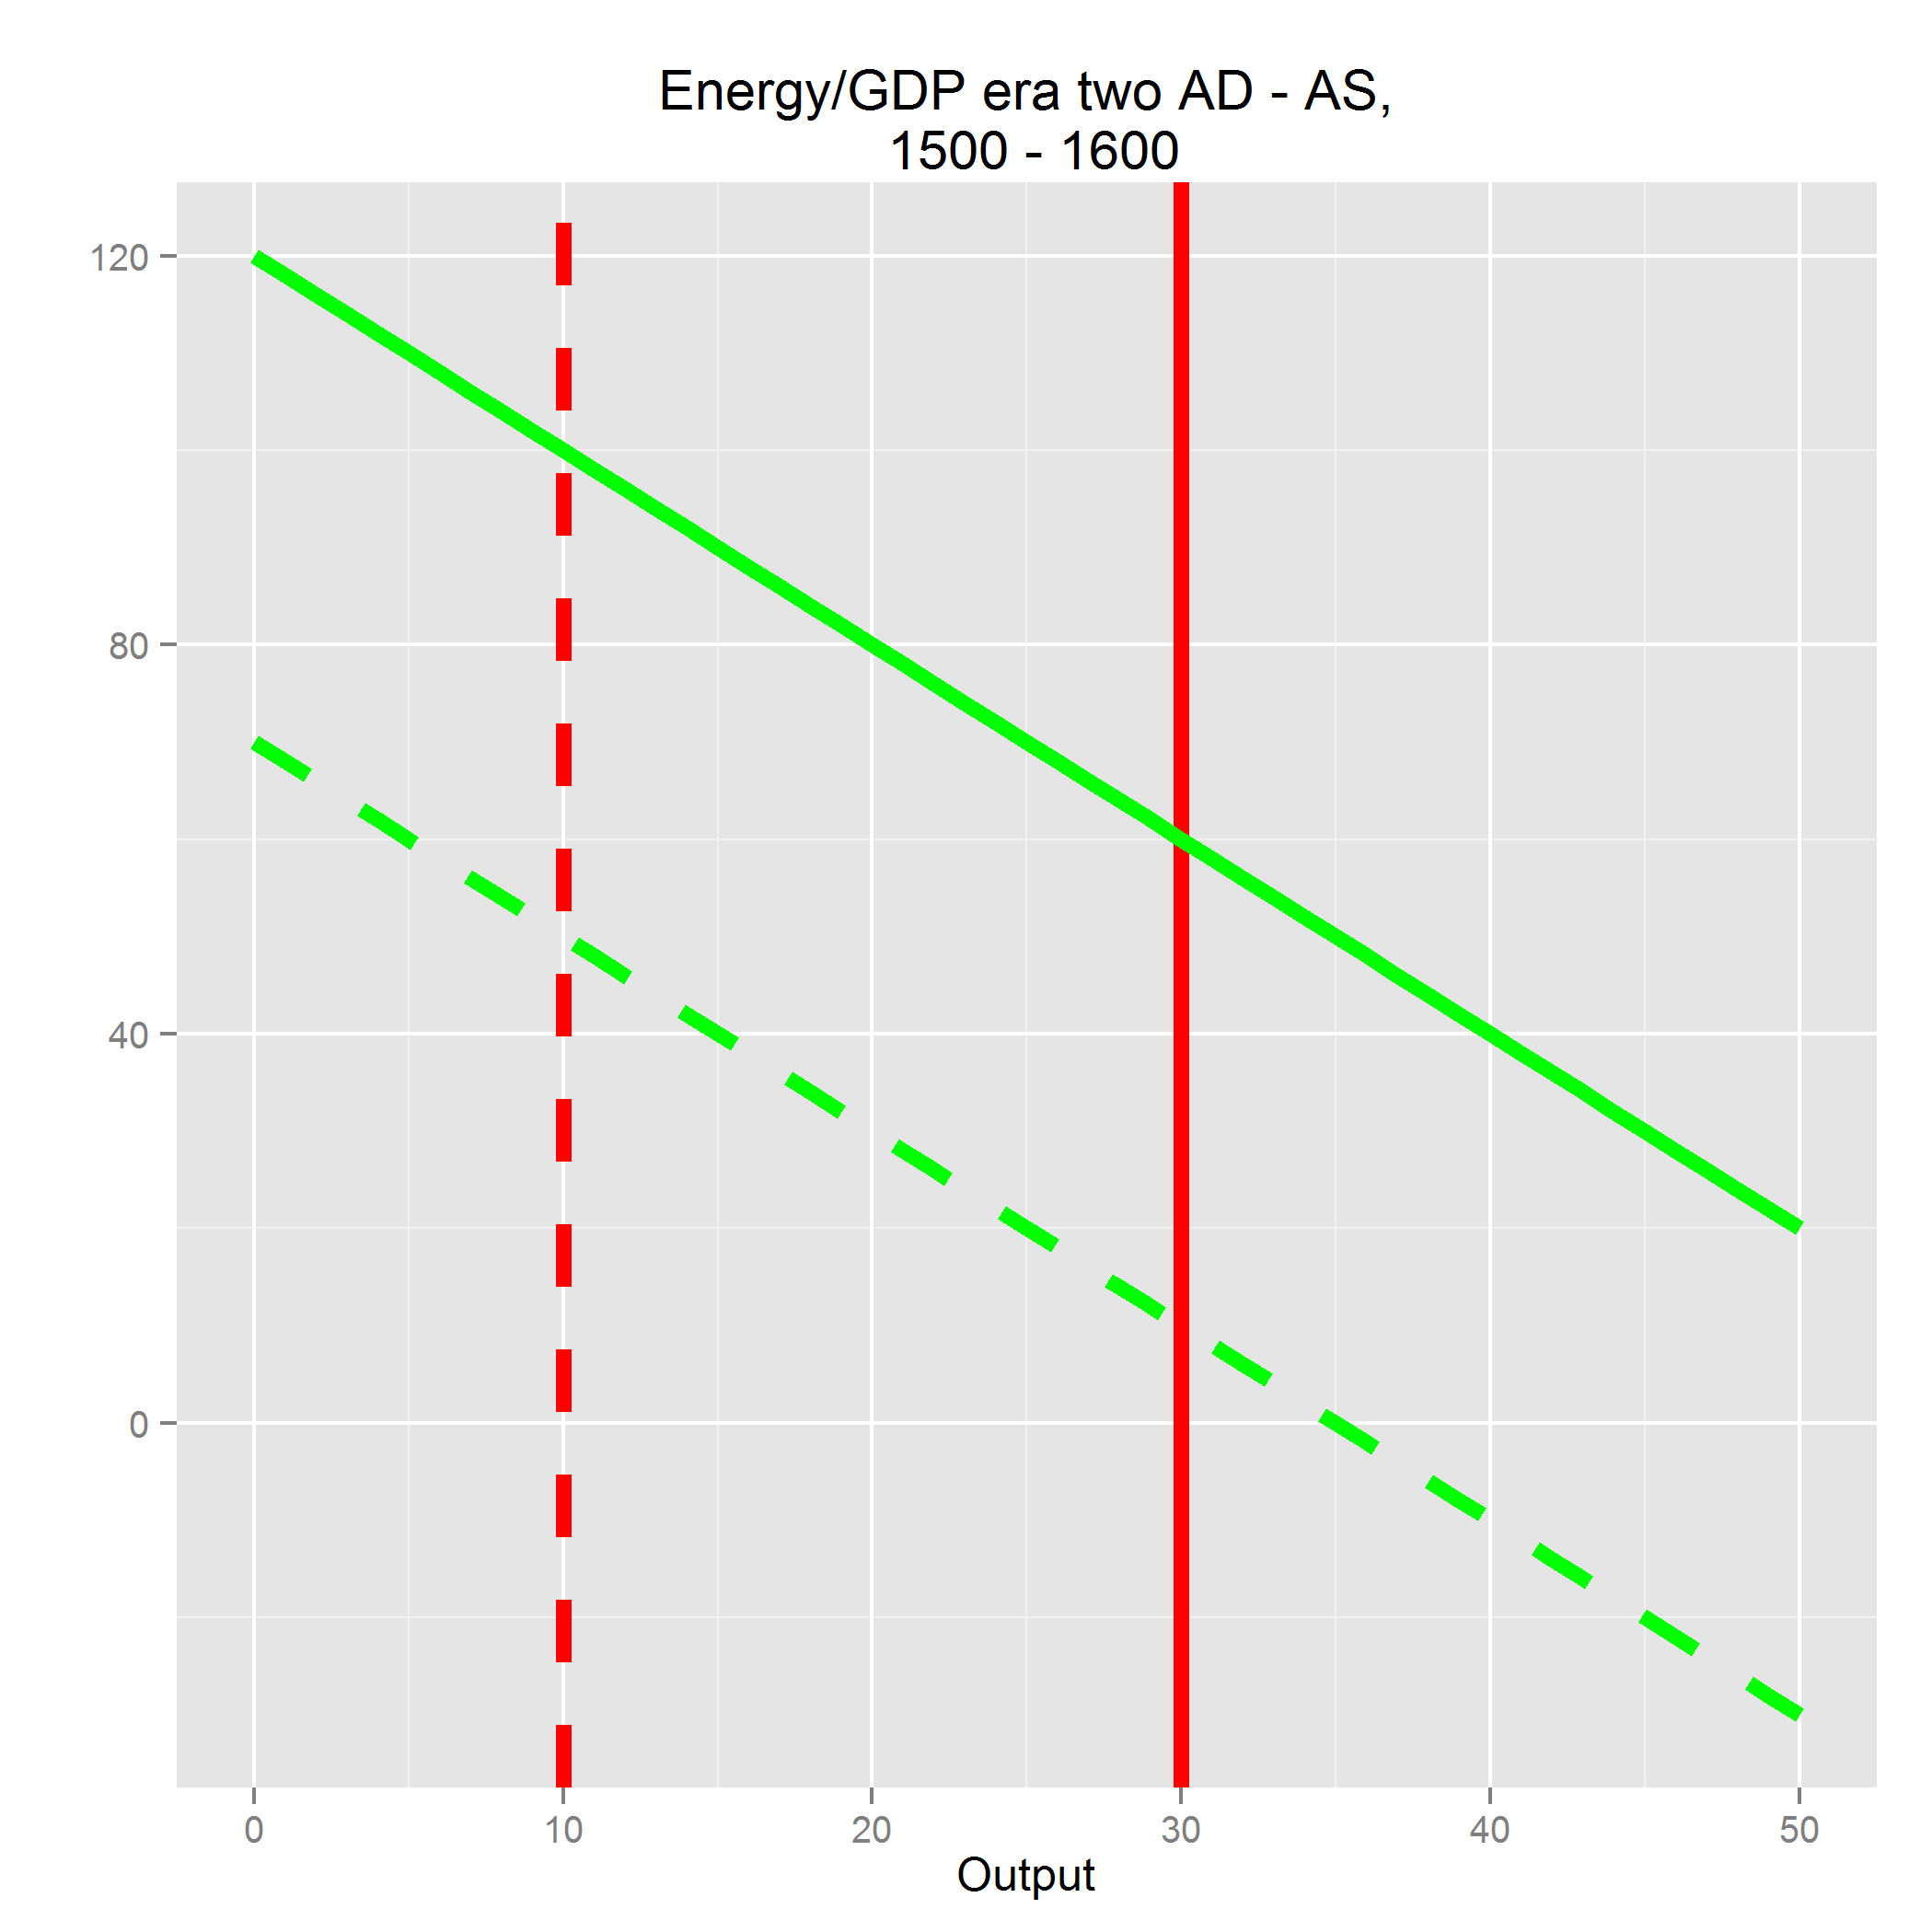
\includegraphics[height=0.35\textheight]{era2}}
		}
		\end{figure}
\begin{figure}[p!]
%		\caption{Aggregate Supply - Aggregate Demand \\ Four energy/GDP regimes}
		\label{fig:asad}		
		\centerline{
		\mbox{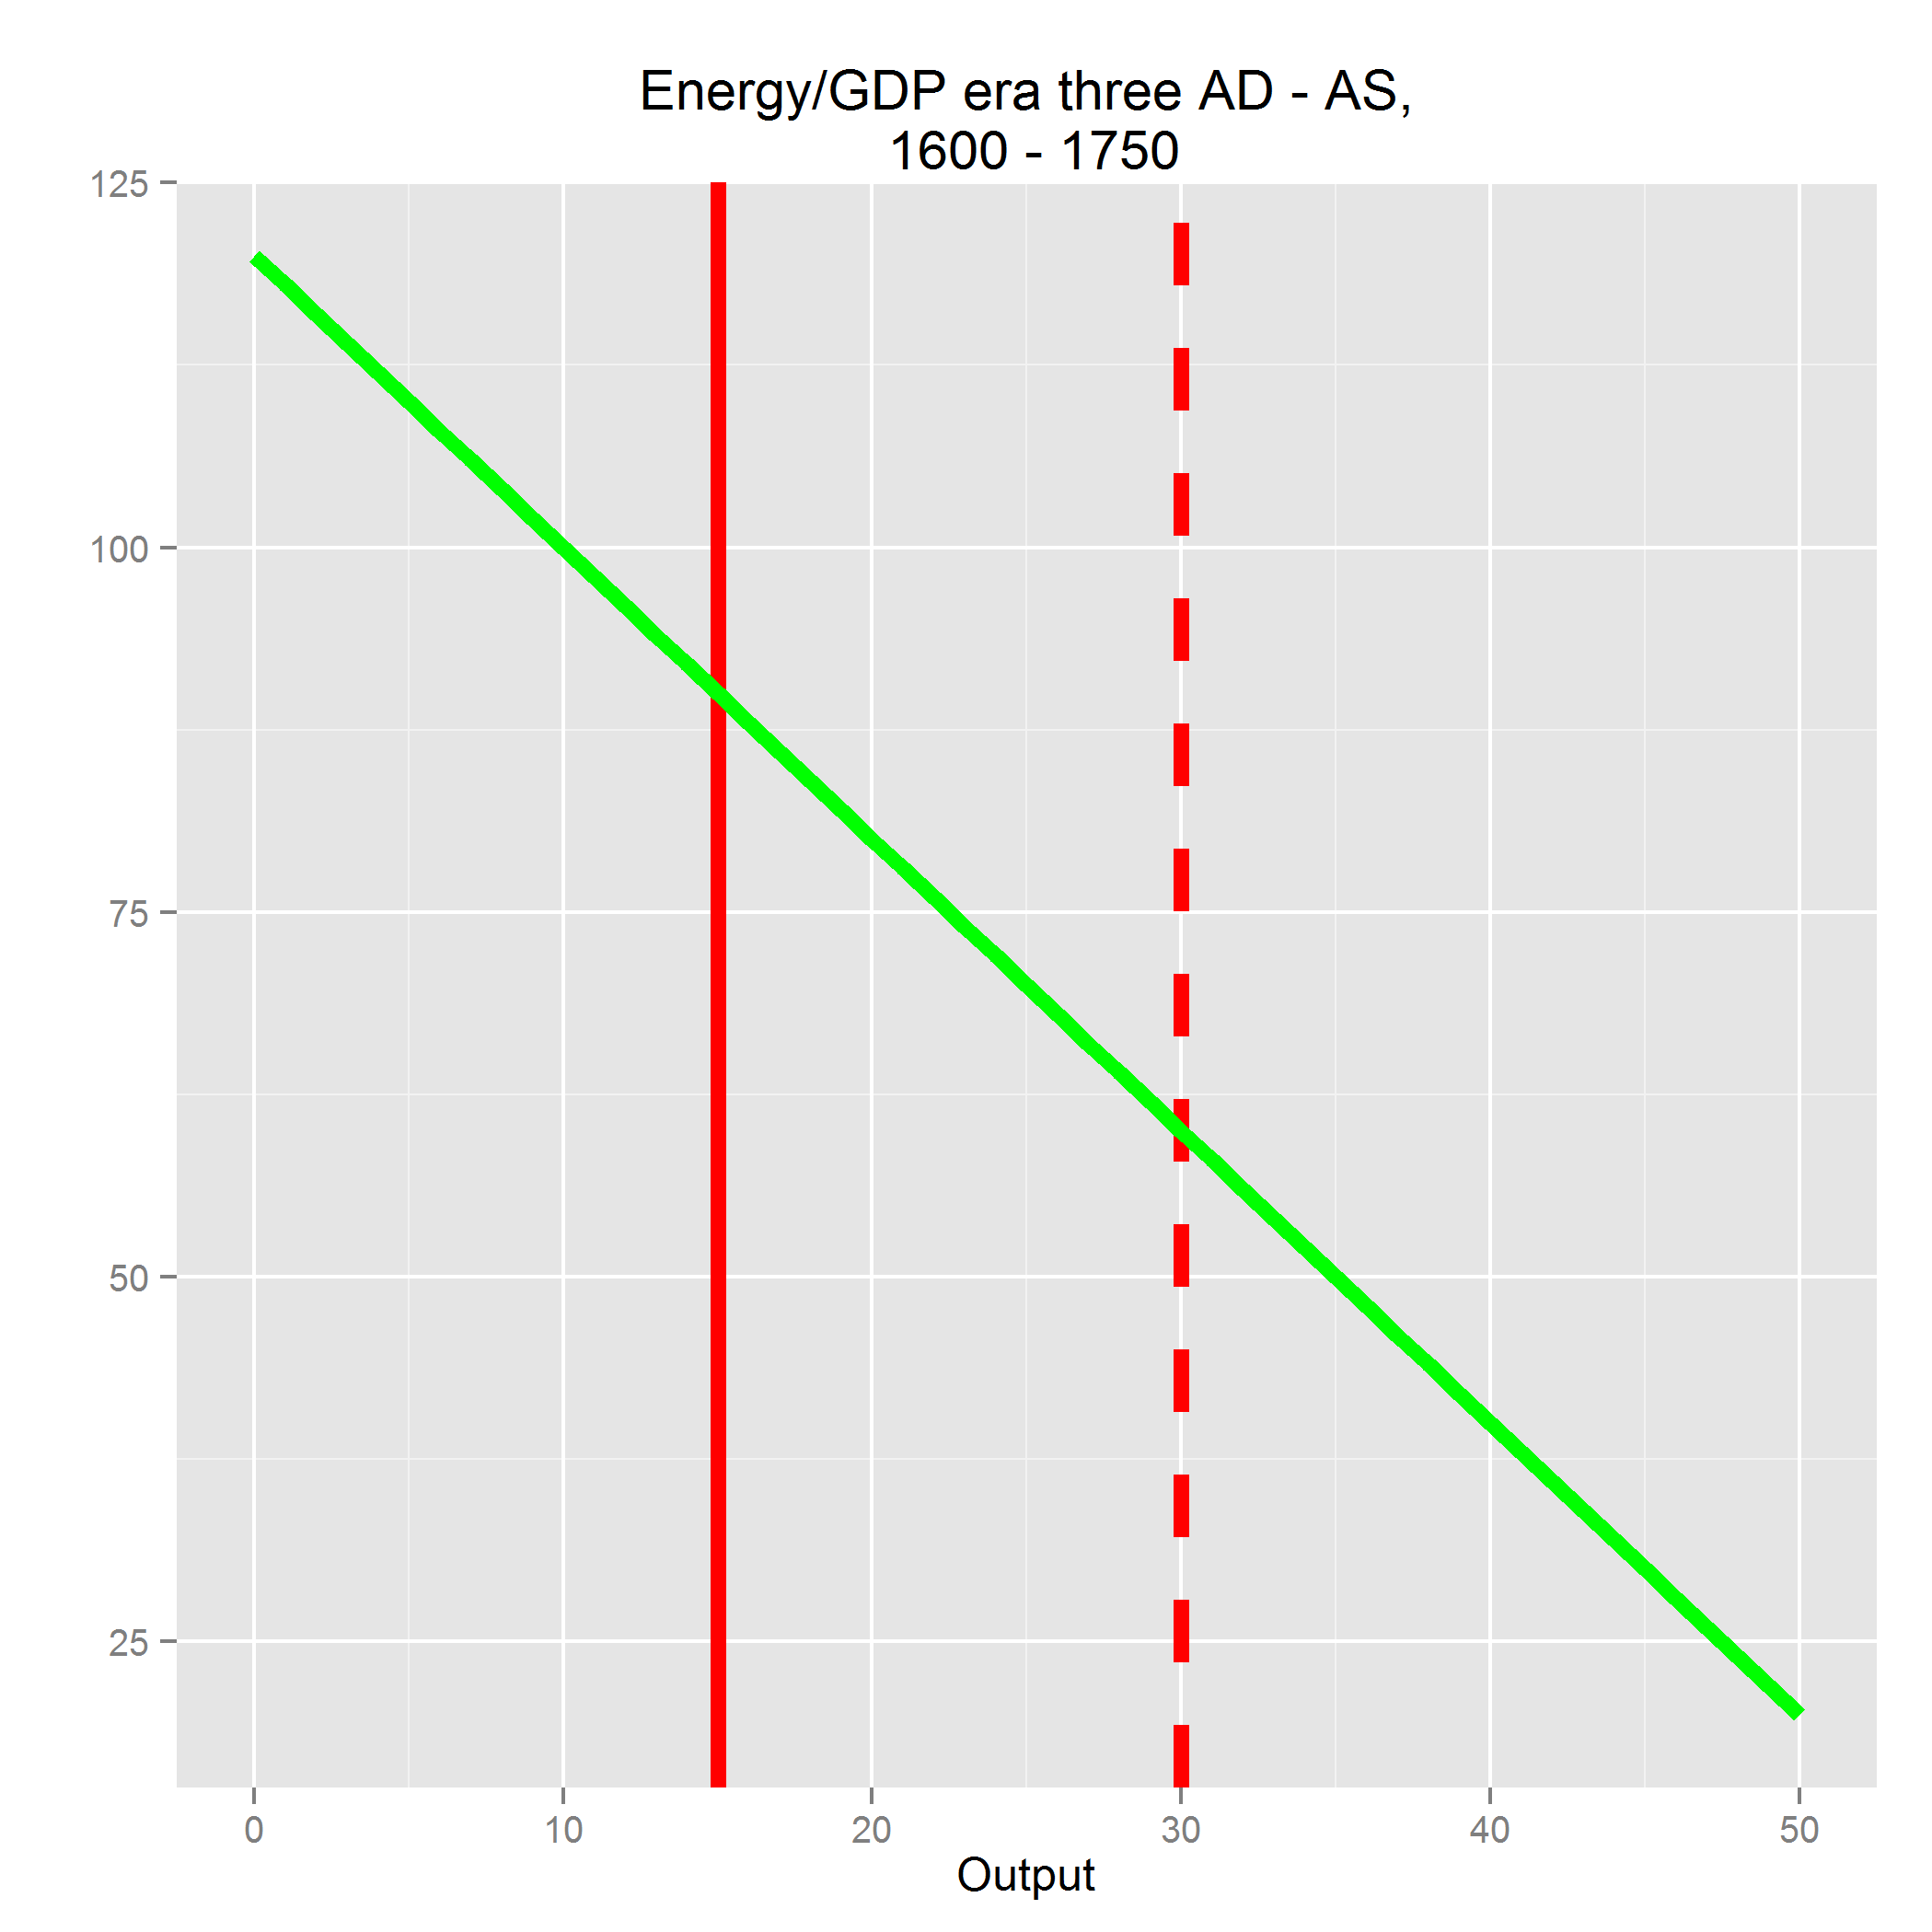
\includegraphics[height=0.35\textheight]{era3}}
		\mbox{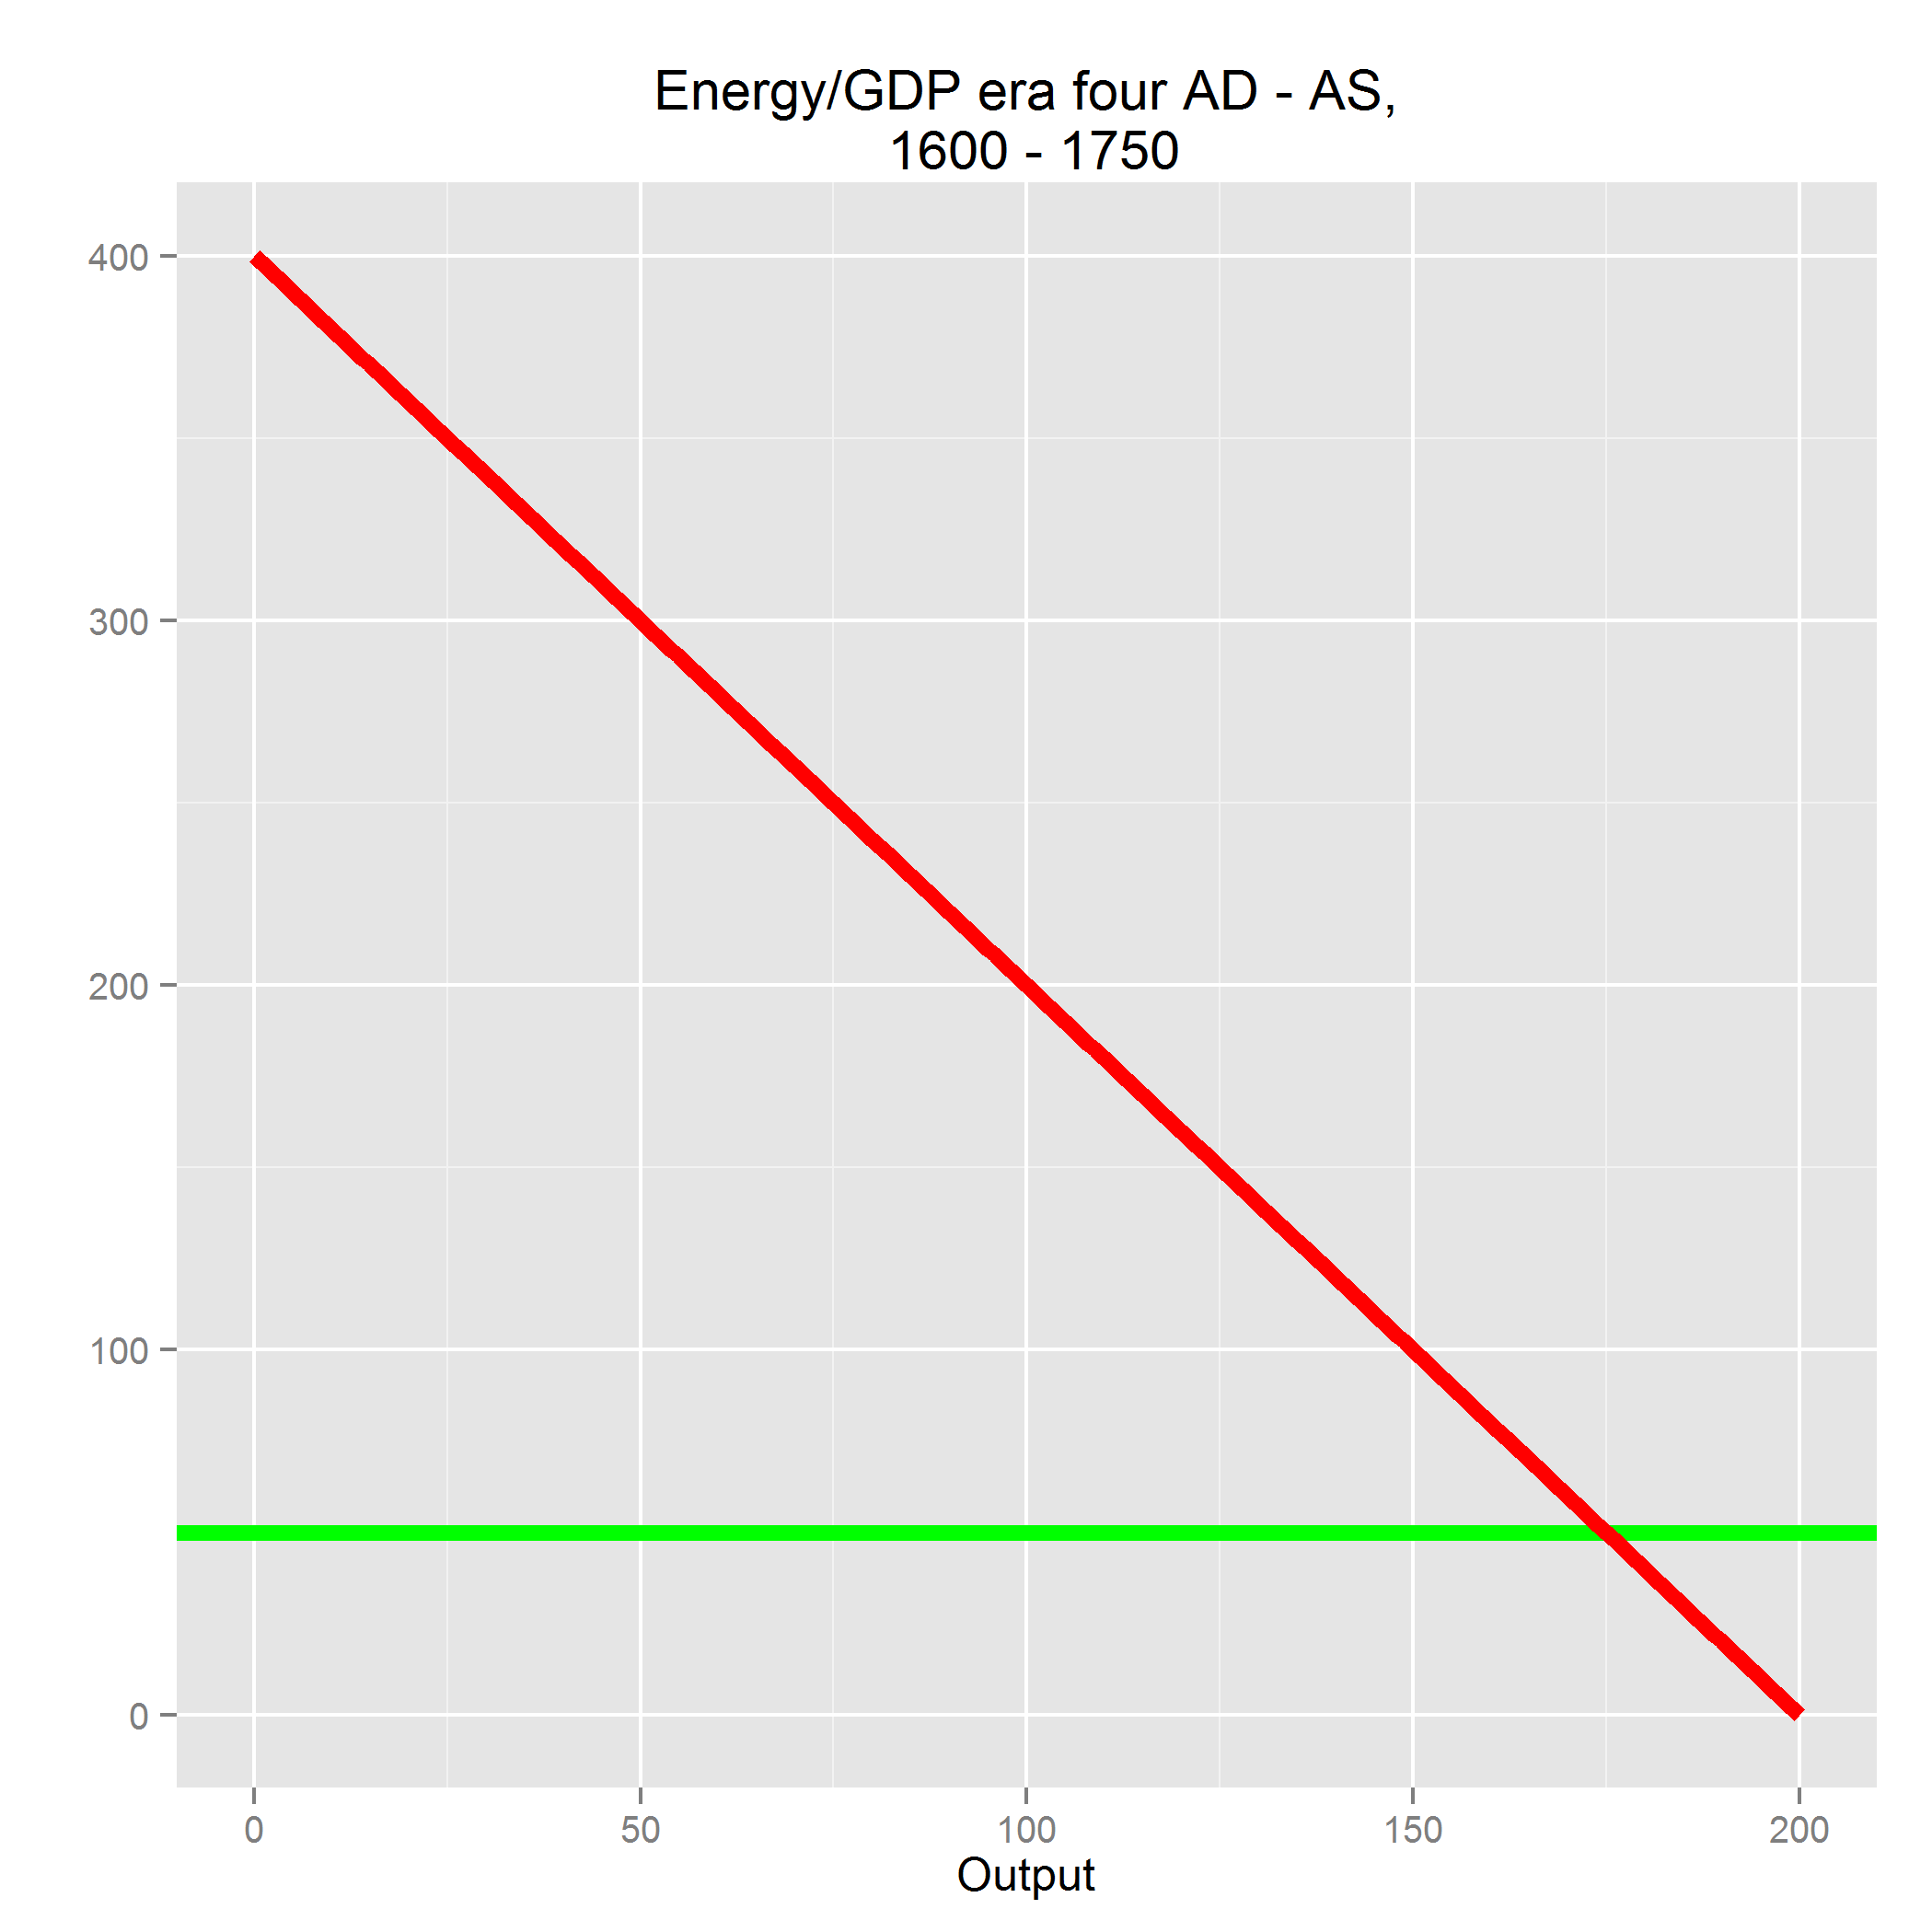
\includegraphics[height=0.35\textheight]{era4}}				
		}
		\end{figure}
\end{frame}


\begin{frame}
		\frametitle{Desaguliers manuscript}
\begin{figure}[p!]
%		\caption{Desaguliers manuscript}
		\label{fig:desagulier}		
		\center
%		\mbox{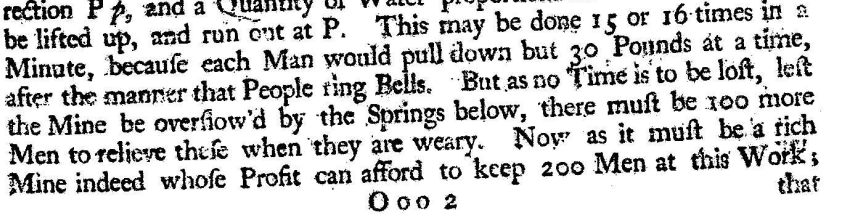
\includegraphics[width=0.95\textwidth]{desagulier1}}\\
%		\mbox{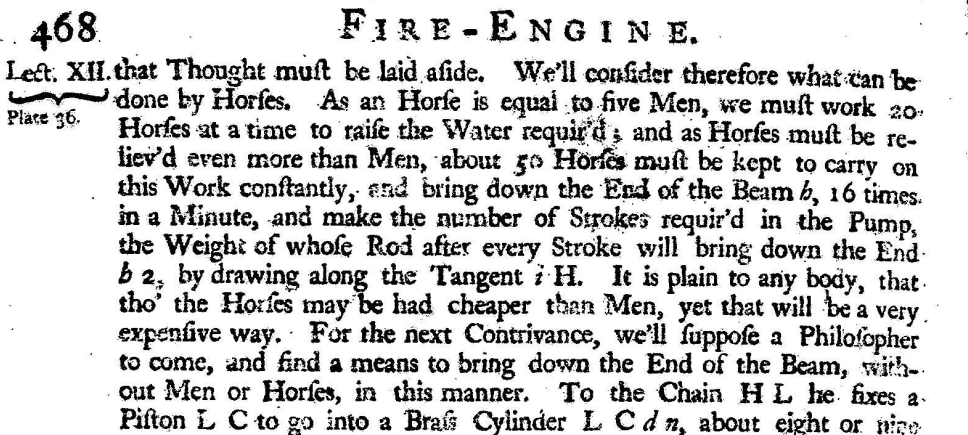
\includegraphics[width=0.95\textwidth]{desagulier2}}
		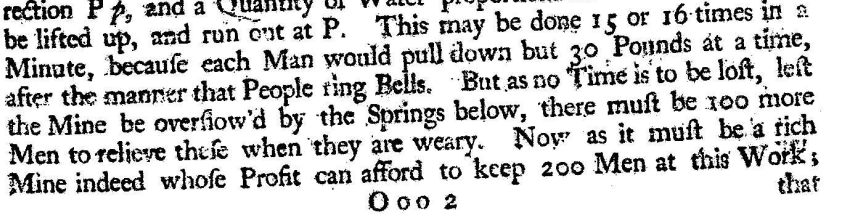
\includegraphics[width=0.95\textwidth]{desagulier1}\\
		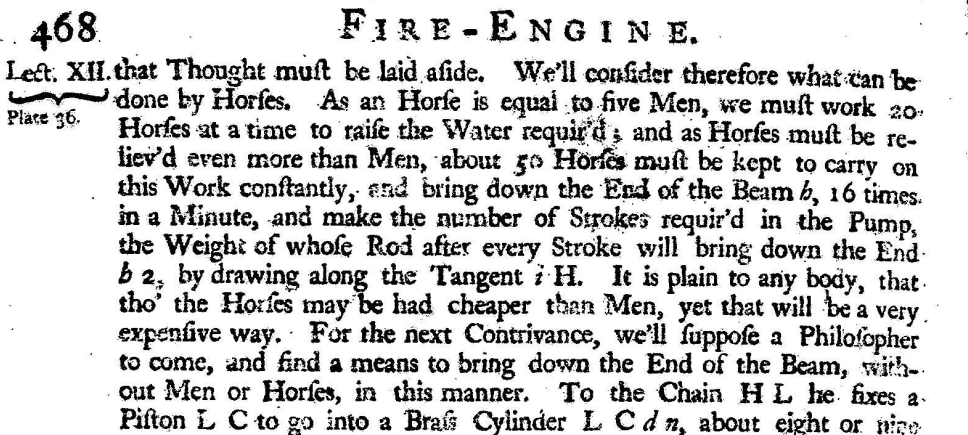
\includegraphics[width=1.05\textwidth]{desagulier2}
%		}
\end{figure}
\end{frame}

\begin{frame}
\frametitle{Real wage to energy ratios\\\textit{Source:} Robert Allen (2009)}
\begin{figure}[p!]
\center
%\caption{Real wage to energy ratios\\\textit{Source:} Robert Allen (2009)}
\label{fig:wage-energy}
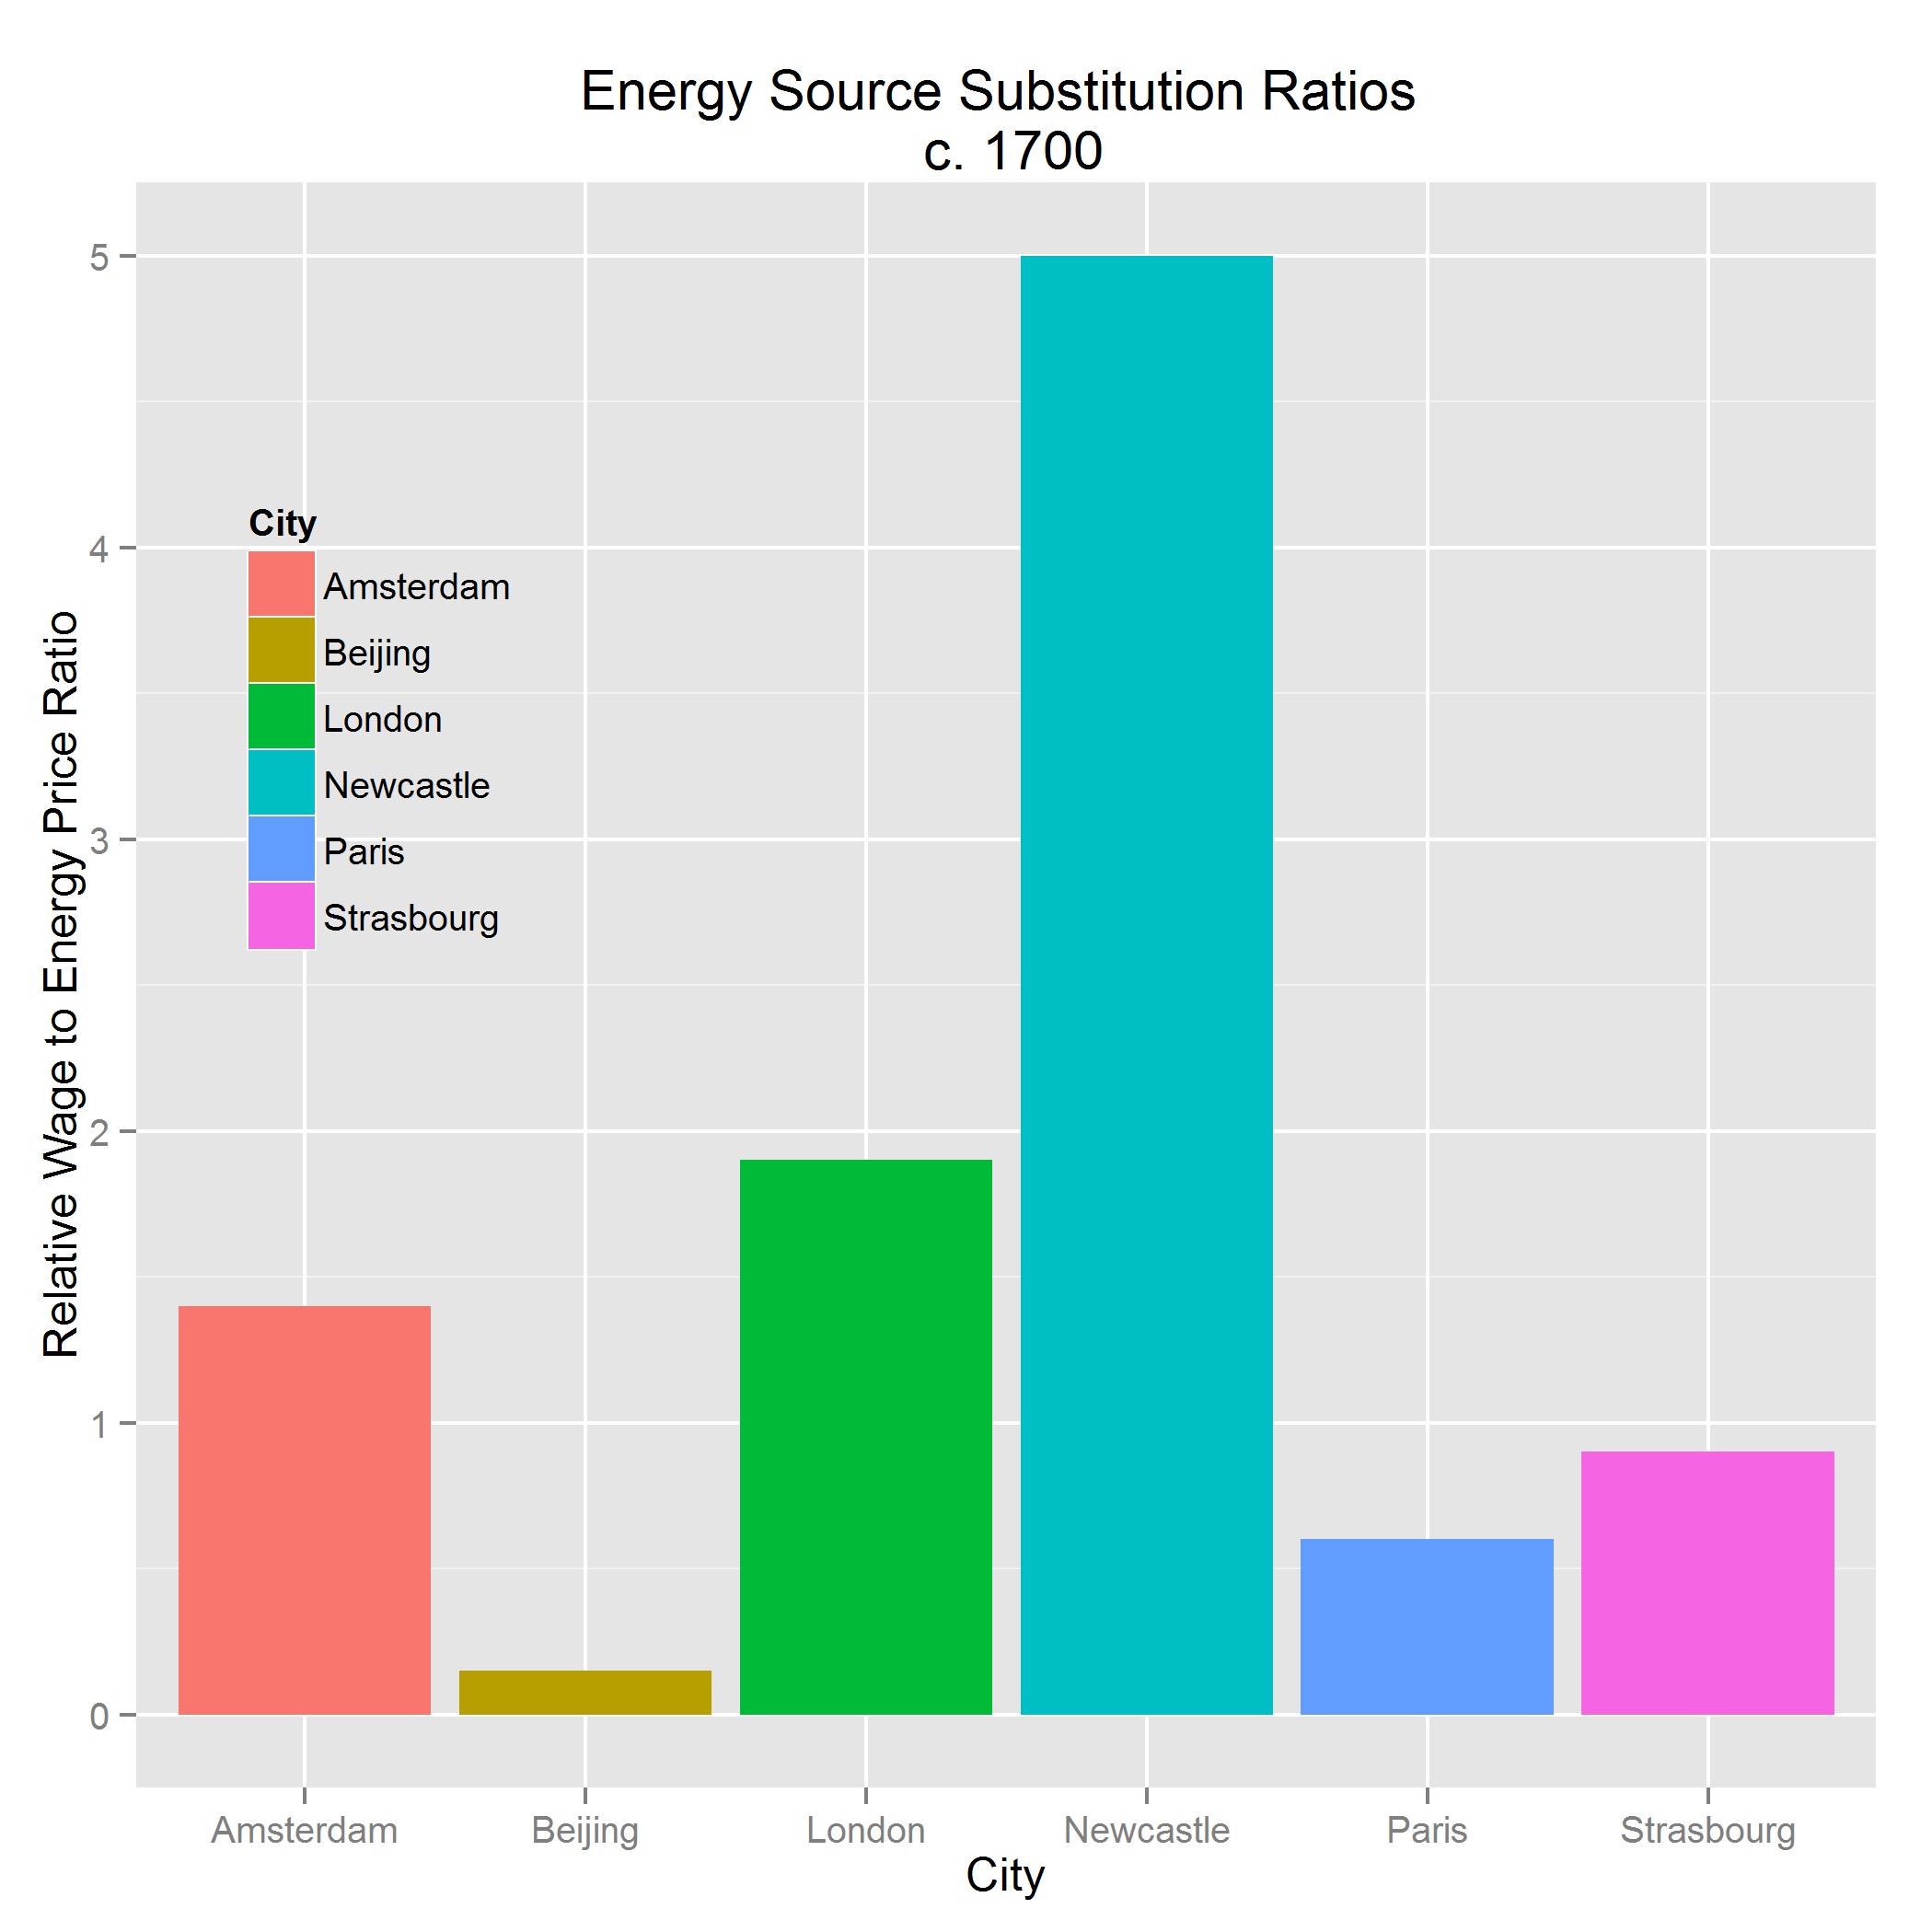
\includegraphics[height=0.8\textheight]{wage-energy.png}
\end{figure}
\end{frame}

\begin{frame}
\frametitle{Microeconomic theory}
\scriptsize{
		\begin{equation}
		\label{eq:mrp}
		\frac{\text{Marginal Revenue Product}_{\text{ organic energy joule}}}{\text{Price}_{\text{ organic energy joule}}} = \frac{\text{Marginal Revenue Product}_{\text{ fossil energy joule}}}{\text{Price}_{\text{ fossil energy joule}}}
		\end{equation}
}
\end{frame}

\begin{comment}
\begin{frame}
\frametitle{English Industrial Revolution, 1590 - 1876}

	\begin{itemize}
	\item Modern economic growth
	\item Unconstrained quantity of fossil carbon energy -- an \textit{energy} revolution led by a demand revolution
	\item Little statistical space for institutional or cultural events -- except to explain structural breaks
	\item Macro and micro explain a great deal
	\item Framework applicable across time series, space, and time
	\end{itemize}
\end{frame}
\end{comment}

\section{Supplement}

\begin{frame}
\frametitle{English wood energy supply constraint}
\begin{figure}[p!]
\center
%\caption{English wood enegy supply constraint}
\label{fig:wood}
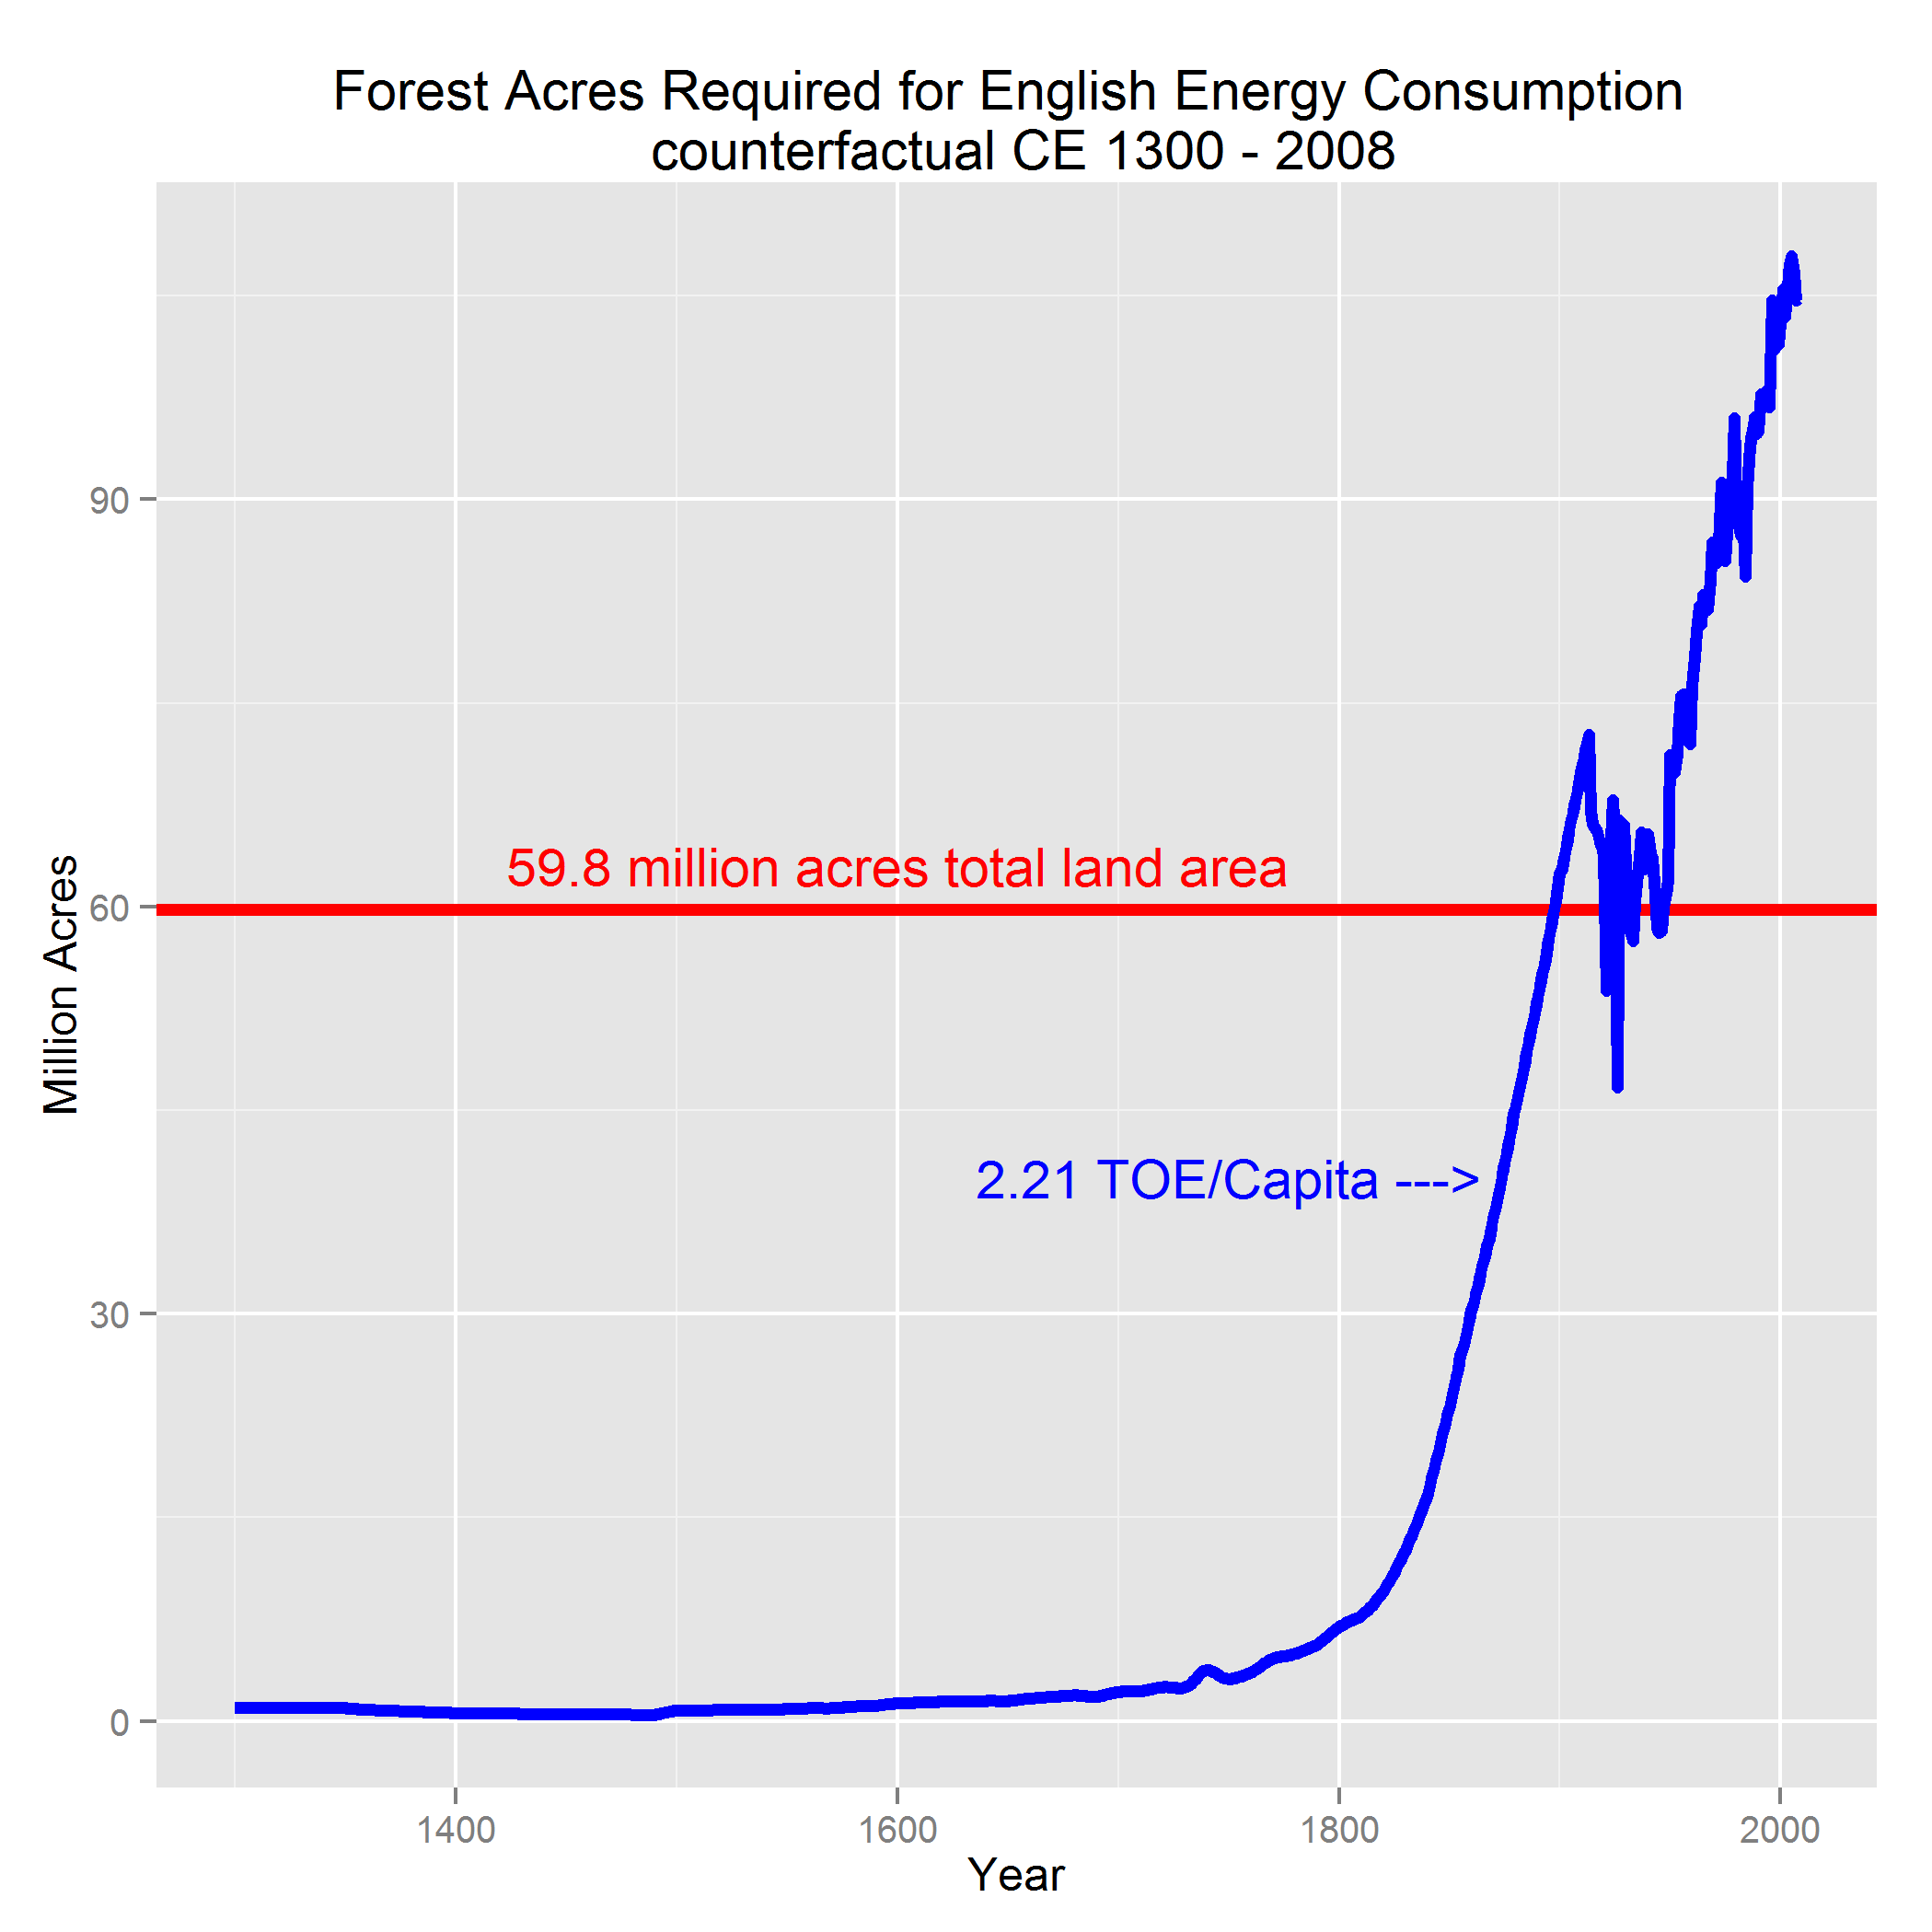
\includegraphics[height=0.8\textheight]{wood}
\end{figure}
\end{frame}

\begin{frame}
\frametitle{The role of AIAS in future economic systems}
\begin{itemize}
\item There is no (economic) activity without energy input, it is the only non-substitutable input \pause
\item Spacetime energy, essentially unlimited and free, will propel us into a new economic regime \pause
\item Andrea Rossi may be able to commercialize LENR without theoretical support, but such support will affect the speed of acceptance \pause
%\item I personally believe if Alex Hill wants to go big with his technology, theoretical support is crucial
\item At the moment, I am trying to be the economic historian who best explains the EIR, on my way to being the economist of space-energy economics \pause
\item What can I do to help?
\end{itemize}
\end{frame}


\begin{frame}
\begin{figure}[p!]
\center
\caption{Standardized English energy intensity of GDP}
\label{fig:energyIntensity}
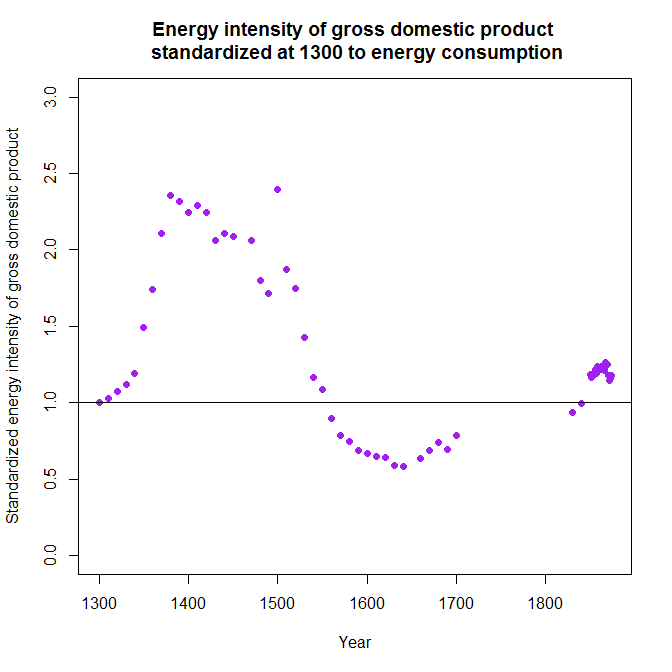
\includegraphics[height=0.8\textheight]{energyIntensity}
\end{figure}
\end{frame}

\begin{frame}
\begin{figure}[p!]
\center
\caption{Log of GDP, with structural breaks}
\label{fig:gbpgdplog.png}
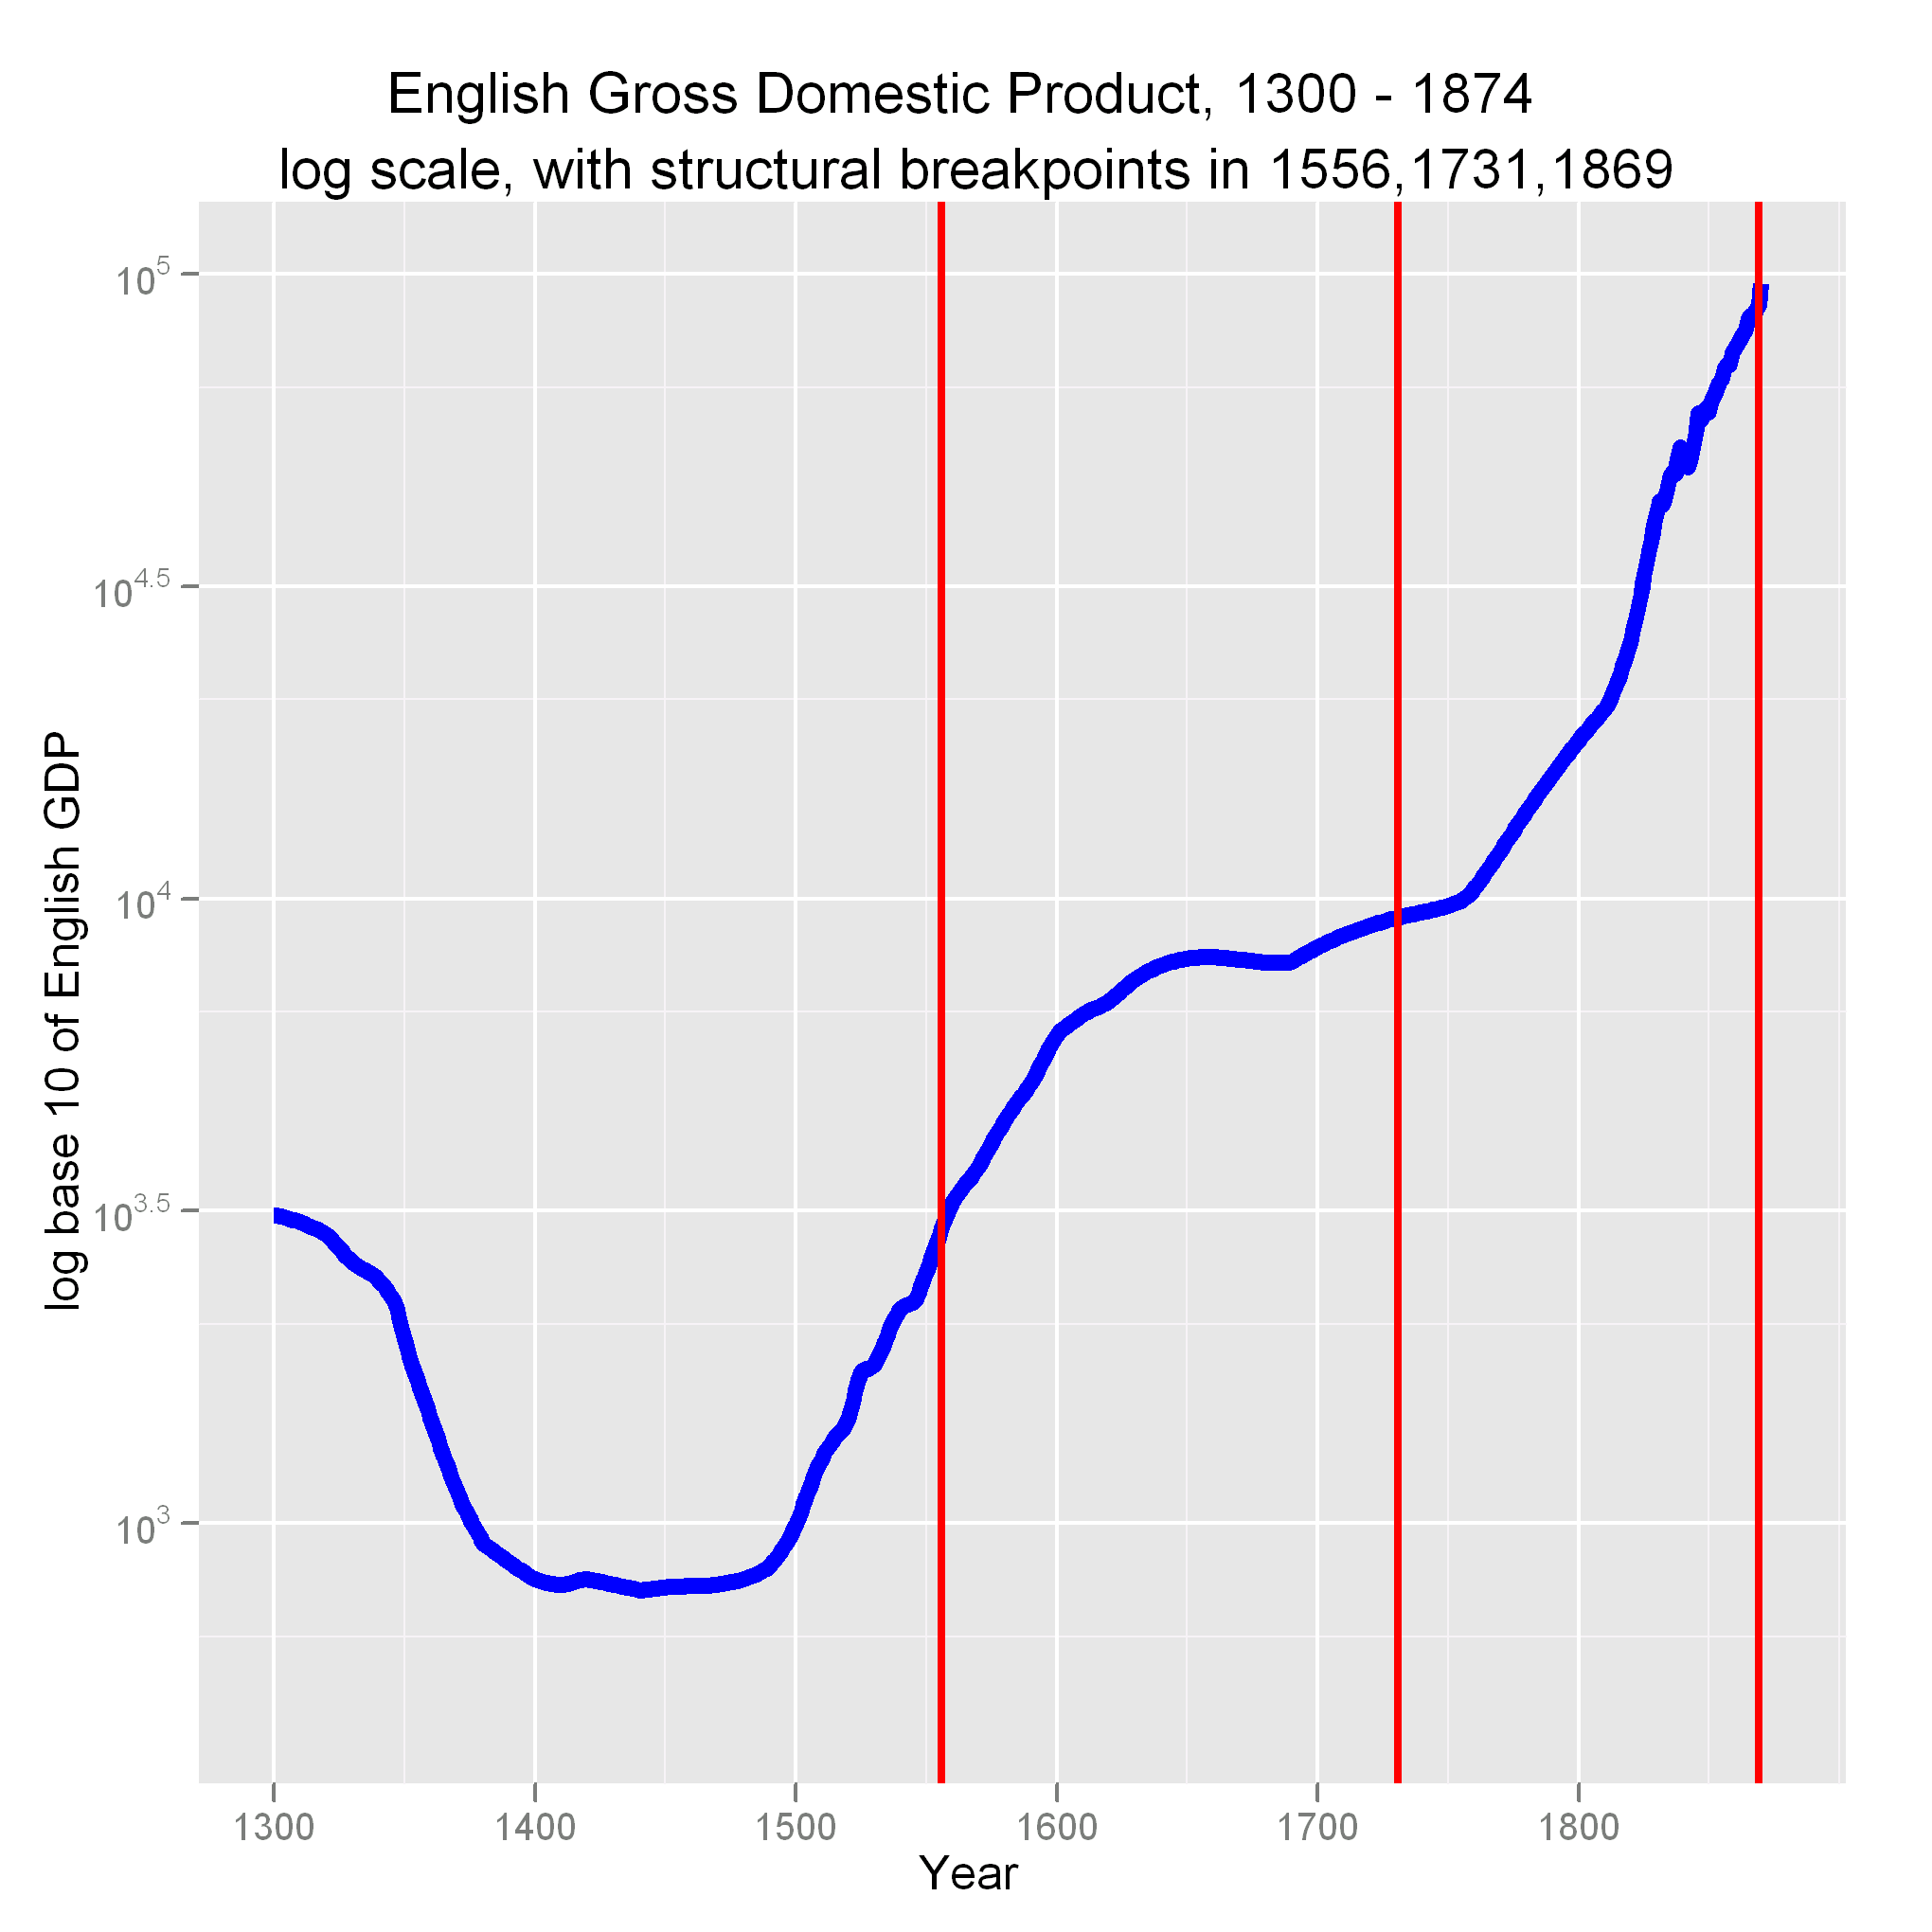
\includegraphics[height=0.8\textheight]{gbpgdplog.png}
\end{figure}
\end{frame}

\begin{frame}
\begin{figure}[p!]
\center
\caption{Log of population, with structural breaks}
\label{fig:popLog}
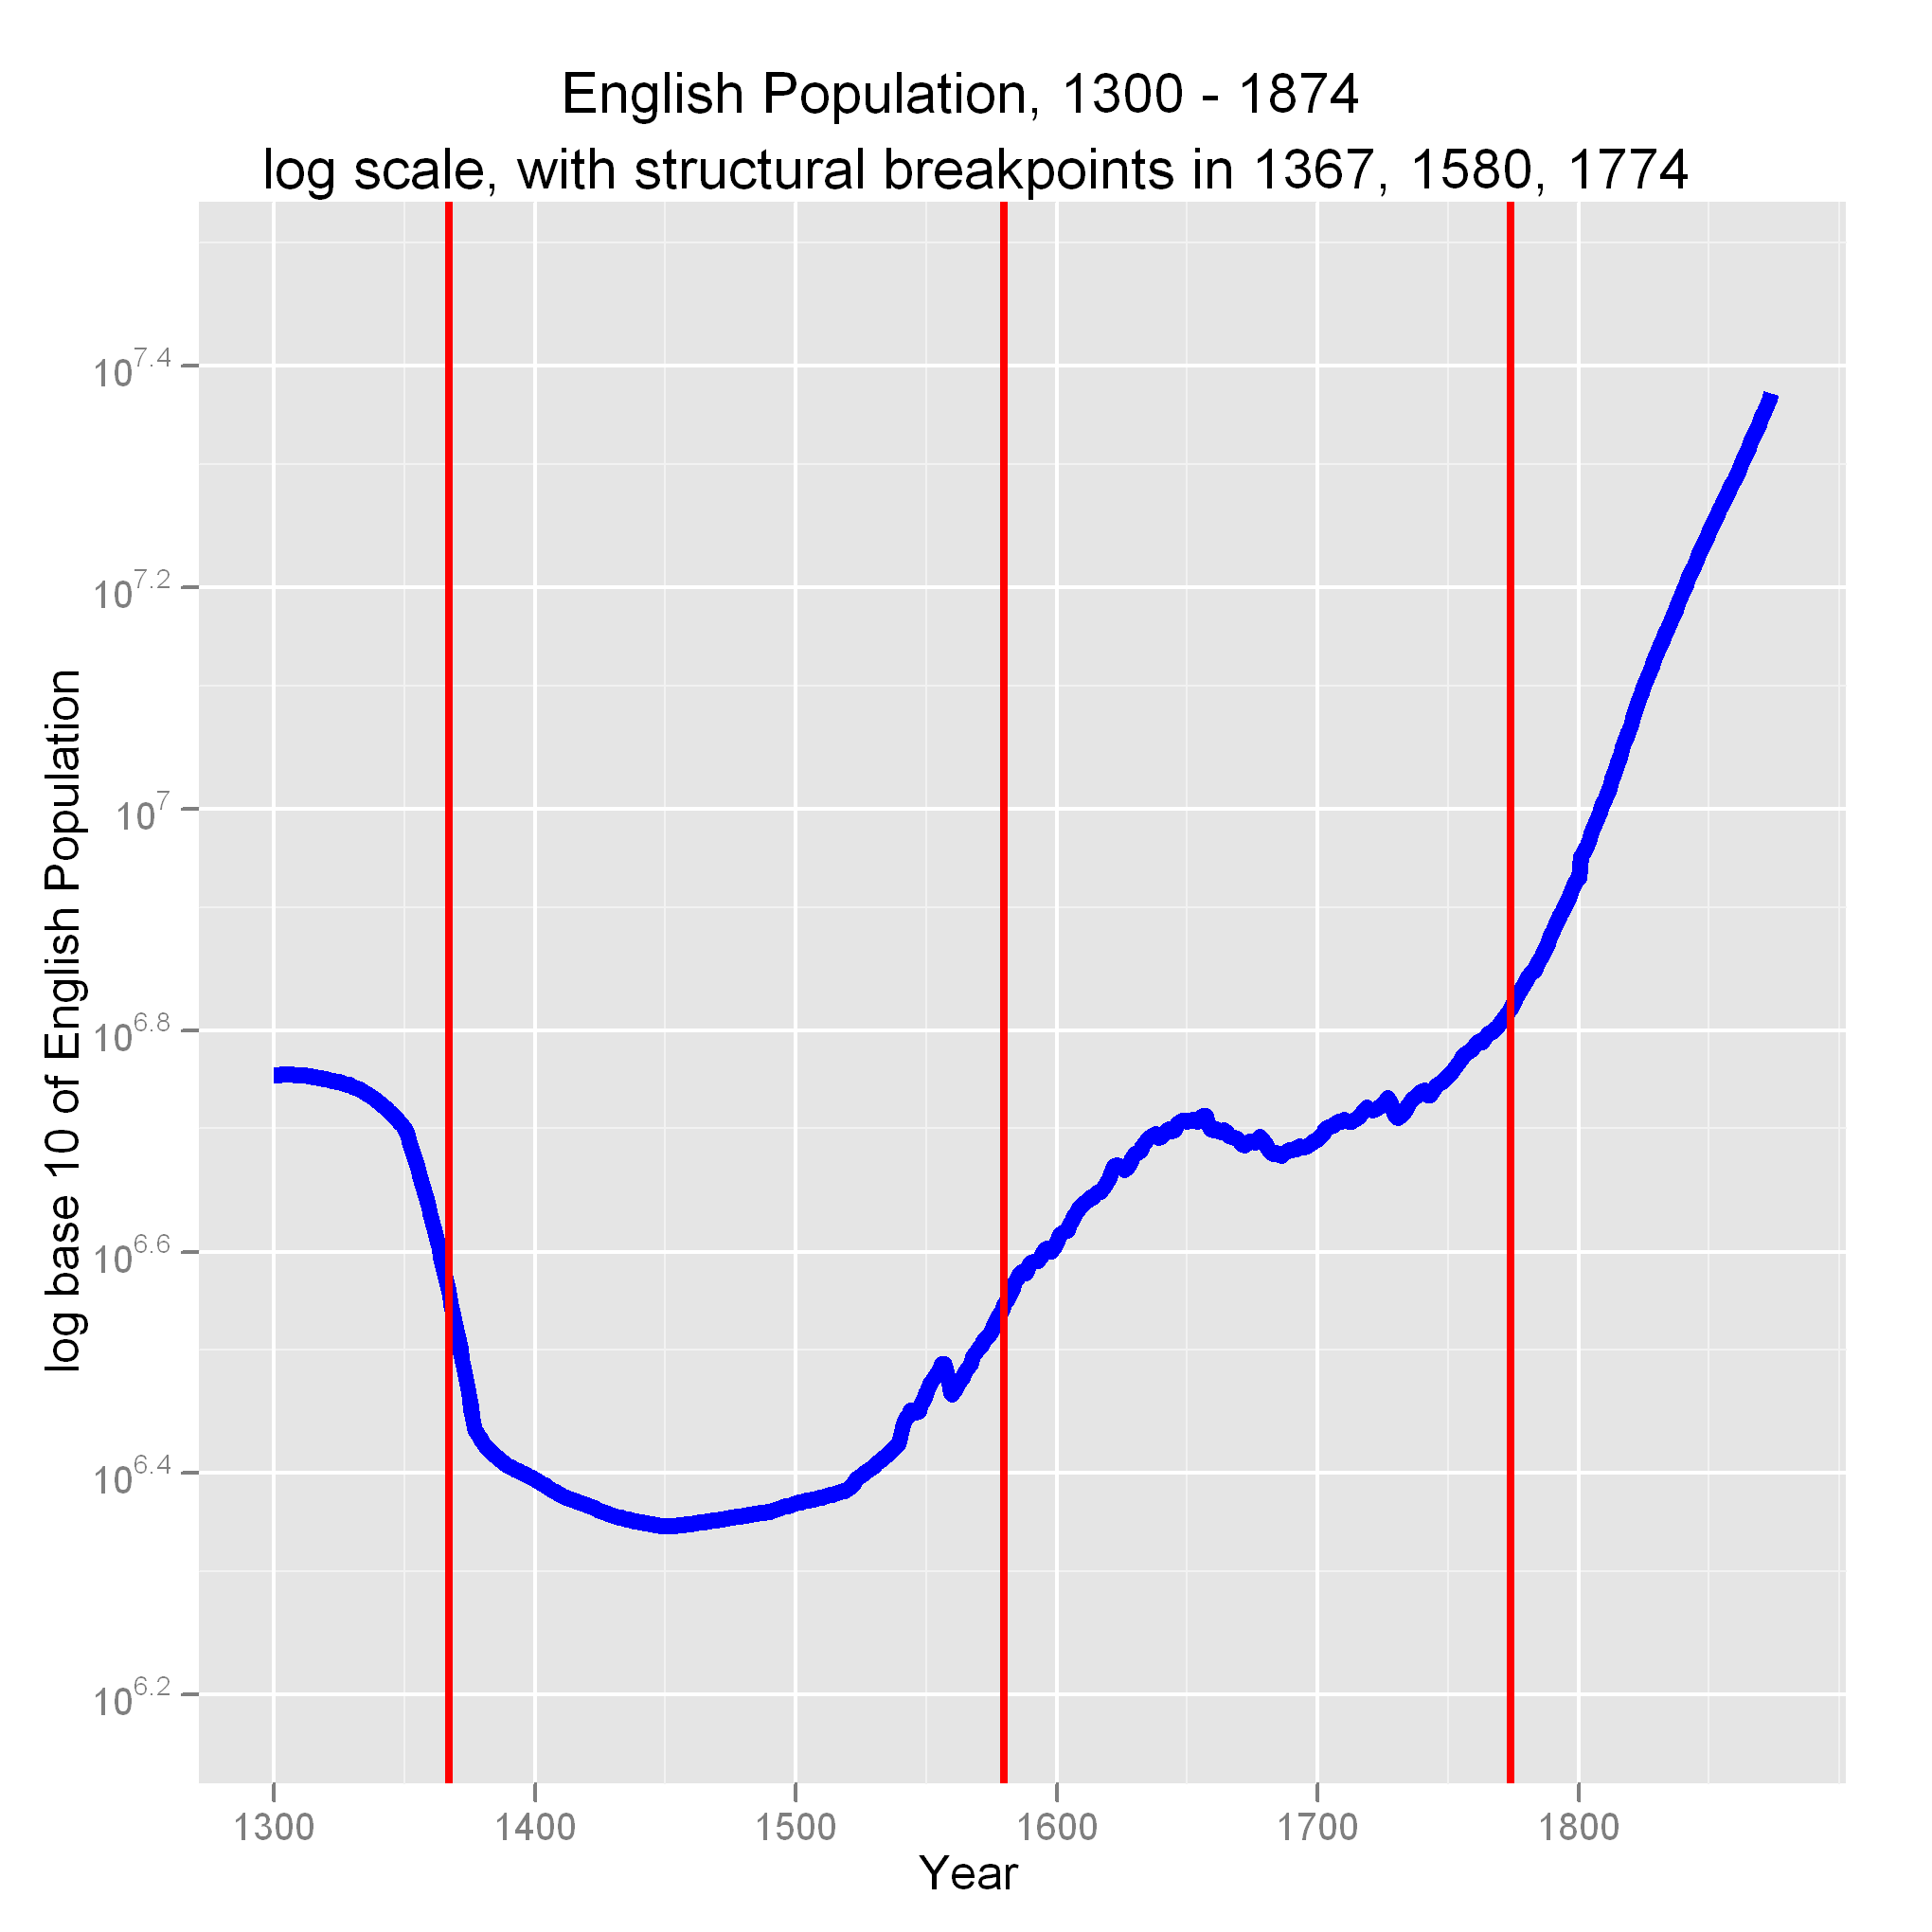
\includegraphics[height=0.8\textheight]{popLog}
\end{figure}
\end{frame}

\begin{frame}
\frametitle{Data Sources}
\footnotesize{
\begin{table}[p!]
%\caption{Data Sources}
\label{tbl:dataSources}
\begin{tabular}{lrll}
Data series&Year range&Geography&Source\\
\hline
Energy consumption&1300 -- 1873&England/Wales&Roger Fouquet (2008)\\
\hline
Gross domestic product&1300 -- 1700&England&Graeme Snooks (1994)\\
&1741 -- 1873&England/Wales&Lawrence Officer (2009)\\
\hline
Population&1300 -- 1540&England&Graeme Snooks (1994)\\
&1541 -- 1800&England&B. R. Mitchell (1988)\\
&1801 -- 1873&England/Wales&B. R. Mitchell (1988)\\
\end{tabular}
\end{table}
}
\end{frame}

\begin{comment}
\begin{table}[p!]
\caption{t-test of energy and gdp}
\label{tbl:t-testEnergyGdp}
\begin{tabular}{rl}
\end{tabular}
\end{table}
\end{comment}

\begin{frame}
\tiny{
\begin{table}[p!]
\caption{growth rates by century}
\label{tbl:growthByCentury}
\begin{tabular}{lrrrrrrrr}
Year	&	1300	&	1400	&	1500	&	1600	&	1700	&	1801	&	1873&Total	\\
\hline
GDP Million\\ 2005 GBP	&	3114.7541	&	815.1288	&	994.4571	&	6031.953	&	8361.5911	&	18110	&	102811&	\\
Century-over-century\\rate of growth&&-0.738&0.220&5.066&0.386&1.166&4.677&32.008\\
Compounded annual \\rate of growth&&-0.013&0.002&0.018&0.003&0.008&0.024&0.006\\
\hline
Energy consumption&1.7	&	1	&	1.3	&	2.2	&	3.6	&	11.6	&	66.1&	\\
Century-over-century\\rate of growth&&-0.412&0.300&0.692&0.636&2.222&4.698&37.882\\
Compounded annual \\rate of growth&&-0.005&0.0026&0.005&0.005&0.012&0.024&0.006\\
\hline
Per-capita GDP\\2005 GBP&542&  329&  421& 1,484& 1,663& 1,999& 4,392\\
Century-over-century\\rate of growth&&-0.393& 0.282&2.521&0.121&0.202&1.198& 7.108\\
Compounded annual \\rate of growth&&-0.005&0.002&0.013&0.001&0.002& 0.011&0.004\\
\end{tabular}
\end{table}
}
\end{frame}

\begin{frame}
\begin{table}[p!]
\caption{Energy and GDP fit tests}
\label{tbl:fitTest}
\begin{center}
\begin{tabular}{lrr}
\hline\hline
Test&Statistic&p-value\tabularnewline
\multicolumn{1}{c}{}\tabularnewline
\hline
Pearson's correlation&$0.998$&\tabularnewline
\hline
Paired t-test&$5.592$&4.991e-07\tabularnewline
\hline
Chi-square&2864&0.0004998\tabularnewline
\end{tabular}
\end{center}
\end{table}
\end{frame}



\end{document}